% Nejprve uvedeme tridu dokumentu s volbami
\documentclass[czech,bachelor]{diploma}
%asmath  pro matrix jsem potreboval
\usepackage{amsmath}
% pro a b c enumerate
\usepackage{enumitem}
% tikz a barvicky
\usepackage{float} % pro [H] option u figures
% \usepackage{subcaption} % pro grid obrazku
\usepackage{tikz}
% pro grafy
\usepackage{pgfplots}
\pgfplotsset{compat=1.16}
%
\usetikzlibrary{fit,positioning,matrix}
\usepackage{xstring}
% Dalsi doplnujici baliky maker
\usepackage[autostyle=true,czech=quotes]{csquotes} % korektni sazba uvozovek, podpora pro balik biblatex
\usepackage[backend=biber, style=iso-numeric, alldates=iso]{biblatex} % bibliografie
\usepackage{dcolumn} % sloupce tabulky s ciselnymi hodnotami
\usepackage{subfig} % makra pro "podobrazky" a "podtabulky"
\usepackage[cpp]{diplomalst}

% Zadame pozadovane vstupy pro generovani titulnich stran.
\ThesisAuthor{Daniel Slavík}

\ThesisSupervisor{Ing. Tomáš Fabián Ph.D.}

\CzechThesisTitle{Lokalizace klíčových bodů pomocí neuronových sítí}

\EnglishThesisTitle{Keypoint Detection with Neural Networks}

\SubmissionYear{2024}

\ThesisAssignmentFileName{ThesisSpecification_SLA0331_vsboee23037AAD.pdf}

% Pokud nechceme nikomu dekovat makro zapoznamkujeme.
\Acknowledgement{Rád bych poděkoval panu Ing. Tomáši Fabiánovi, Ph.D. za odbornou pomoc a inspiraci při vytváření této bakalářské práce.}

\CzechAbstract{Cílem této bakalářské práce je }

\CzechKeywords{typografie; \LaTeX; diplomová práce}

\EnglishAbstract{This is English abstract. Lorem ipsum dolor sit amet, consectetuer adipiscing elit. Fusce tellus odio, dapibus id fermentum quis, suscipit id erat. Aenean placerat. Vivamus ac leo pretium faucibus. Duis risus. Fusce consectetuer risus a nunc. Duis ante orci, molestie vitae vehicula venenatis, tincidunt ac pede. Aliquam erat volutpat. Donec vitae arcu. Nullam lectus justo, vulputate eget mollis sed, tempor sed magna. Curabitur ligula sapien, pulvinar a vestibulum quis, facilisis vel sapien. Vestibulum fermentum tortor id mi. Etiam bibendum elit eget erat. Pellentesque pretium lectus id turpis. Nulla quis diam.}

\EnglishKeywords{typography; \LaTeX; master thesis}

\AddAcronym{SIFT}{Škálově invariantní transformace charakteristik/rysů, Scale-invariant feature transform}
\AddAcronym{CNN}{Konvoluční neuronová síť, Convolutional Neural Network}
\AddAcronym{FCN}{Plně konvoluční síť, Fully Convolutional Network}
\AddAcronym{DNN}{Hluboká neuronová síť, Deep Neural Network}
\AddAcronym{PnP}{Perspektiva a bod, Perspective-n-Point}
\AddAcronym{DoF}{Dimenze svobody, Degrees of Freedom}
\AddAcronym{DoG}{Rozdíl Gaussiánu, Difference of Gaussian}
\AddAcronym{PSP}{Schéma pyramidové parsování, Pyramid Scheme Parsing}
\AddAcronym{HSV}{Odstín Sytost Hodnota, Hue Saturation Value}
\AddAcronym{STN}{Neuronová síť s prostorovým transformerem, Spatial Transformer Network}
\AddAcronym{RGB}{Červená zelená modrá, Red Green Blue}
\AddAcronym{ReLU}{Rektifikovaná lineární jednotka, Rectified Linear Unit}
\AddAcronym{YOLO}{Podíváš se pouze jednou, You Only Look Once}
\AddAcronym{JPEG}{Joint Photographic Experts Group}
\AddAcronym{CSV}{Čárkou oddělené hodnoty, Comma-separated values}
\AddAcronym{BN}{Dávková normalizace, Batch Normalization}
\AddAcronym{MSE}{Střední kvadratická chyba, Mean Squared Error}
\AddAcronym{VRAM}{Video paměť, Video Random Access Memory}
\AddAcronym{KDE}{Odhad hustoty statistickým oknem, Kernel Density Estimator}

\addbibresource{biblatex.bib}

% Novy druh tabulkoveho sloupce, ve kterem jsou cisla zarovnana podle desetinne carky
\newcolumntype{d}[1]{D{,}{,}{#1}}


% Zacatek dokumentu
\begin{document}

% Nechame vysazet titulni strany.
\MakeTitlePages

% Jsou v praci obrazky? Pokud ano vysazime jejich seznam a odstrankujeme.
% Pokud ne smazeme nasledujici dve makra.
\listoffigures
\clearpage

% Jsou v praci tabulky? Pokud ano vysazime jejich seznam a odstrankujeme.
% Pokud ne smazeme nasledujici dve makra.
\listoftables
\clearpage

\hyphenation{TensorFlow}


% A nasleduje text zaverecne prace.
\chapter{Úvod}
\label{sec:Introduction}

\begin{figure}[H]
\centering
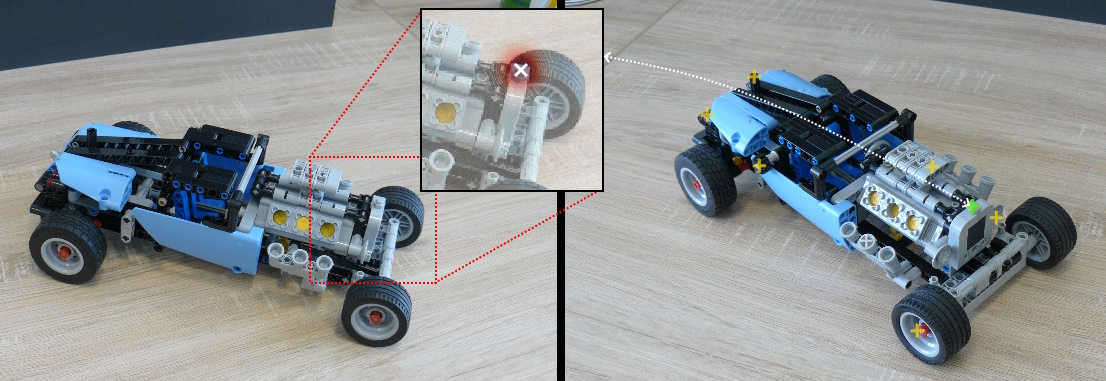
\includegraphics[width=1.0\textwidth,keepaspectratio]{Figures/bp_uvodni_obrazek.jpg}
\caption[Lokalizace klíčového bodu pro řešení PnP problému]{Lokalizace jednoho z klíčových bodů pro řešení PnP problému mezi reálným snímkem (vlevo) a syntetickým vykreslením (vpravo) se známými pozicemi klíčových bodů.}
\label{fig:bp_uvodni_obrazek}
\end{figure}


Lokalizace klíčových bodů zůstává nadále jedním z aktivně řešených problémů analýzy obrazu dnešní doby.
Klíčové body chápeme jako konkrétní body nacházející se na objektu zájmu, které chceme lokalizovat a následně sadu nalezených klíčových bodů použít pro další zpracování tykající se daného objektu zájmu, či jeho částí.

Využití lokalizace bodů nacházíme kupříkladu při odhadu postoje osob \cite{humanpose} nebo v biomedicínské technice \cite{unet}.
Při jejich následné lokalizaci musíme počítat s několika kvalitativně ovliňujícími členy v obrazu jako např. natočení kamery, vzdálenost, osvětlení, charakteristiky a kvalitu obrazu (zaostření) a ostatní vlivy prostředí okolo klíčového bodu. Kvůli tomuto musí techniky pro lokalizaci klíčových bodů být invariantní (tj. odolné vůči změnám ve vzhledu objektů), aby mohly spolehlivě fungovat i během změn vnějších podmínek mezi různými obrazy.

Cílem této bakalářské práce je využít techniky lokalizace klíčových bodů pomocí hlubokých sítí U-Net (a jejími následovníky či variacemi) pro zpřesnění 6 stupňů volnosti (DoF) transformace cílového objektu ve 3D prostoru pomocí PnP metod. PnP metody představují výpočetní techniky určené k řešení PnP problémů, které se zaměřují na přesný odhad polohy a orientace 3D objektů na základě korespondence lokalizovaných klíčových bodů na 2D snímku a známých pozicích klíčových bodů na 3D objektu.

Úloha lokalizace pro část vstupního snímku obsahující klíčový bod je ilustrována pomocí obrázku \ref{fig:bp_uvodni_obrazek}. Pro objekt byl detekován hrubý odhad pozice klíčového bodu. Klíčový bod je pomocí hluboké konvoluční neuronové sítě korektně lokalizován na lokaci s globálním maximem výsledku skalárního pole. Klíčový bod také byl korektně klasifikován s třídou známého klíčového bodu. Za předpokladu korektní lokalizace dostatečného počtu klíčových bodů můžeme orientaci objektu z levé části snímku odhadnout a vyjádřit pomocí 6 stupňů volnosti (DoF).

Výsledná metoda by následně měla být použita pro příjem proud RGB dat z kamery a správně odhadovat pózu objektu v reálném čase. Naše metody řešení budou trénovány na syntetickém datasetu klíčových bodů objektu zájmu a následně porovnány mezi sebou.
\endinput
\chapter{Metody lokalizace klíčových bodů}
\label{sec:Chapter2}
V této kapitole provádíme rešerši na různé metody počítačového vidění pro lokalizaci klíčových bodů. Lokalizaci klíčových bodů na 2D obrázcích můžeme provést klasickými algoritmickými přístupy, jako je například SIFT, který algoritmicky generuje klíčové body na základě distinktivních vlastností obrázků. 

Táto práce se však více bude zaměřovat na využití konvolučních neuronových sítí (CNN) a architektur z řad U-Net pro specializovaně natrénované modely lokalizující klíčové body v řadách desítek milisekund. Následně si také přiblížíme i modul STN, který je možno použít pro adresování problému prostorové invariance v přístupech pomocí konvolučních neuronových sítích.

V této kapitole jsou zmíněny i modely state-of-art, jako je například YOLOv8 či DINOv2, které jsou více obecné a univerzálnější přístupy pro úlohy počítačového vidění v posledních letech.
\endinput
\section{SIFT}
\label{sec:Chapter21}
SIFT -- Scale Invariant Feature Transform (tj. škálově invariantní transformace charakteristik/rysů) představuje jeden z prvních a zároveň klasických metod pro detekci a popis klíčových bodů v obrázcích, jak bylo poprvé popsáno v literatuře \cite{sift}. Tento algoritmus je navržen tak, aby automaticky identifikoval a popsal velké množství klíčových bodů v různých škálách vstupního obrázku, což může dosáhnout počtu v řádech tisíců pro obrázky s rozměry přibližně $500\times500$ pixelů. Přesné množství detekovaných bodů závisí na vizuálních charakteristikách a složitosti obrázku.

Pro lokalizaci bodů se používají vzájemné rozdíly Gaussovy funkce s různými hodnotami sigma ($\sigma$). Tento proces spočívá ve vyhledávání lokálních extrémů v rozdílech mezi sousedními úrovněmi Gaussovy funkce aplikovanými na obrázek v dané škále obrázku (oktávě). SIFT generuje těchto oktáv několik, každý s jinou velikostí daného původního obrázku. Pro každou oktávu je pak vygenerována sada těchto výsledků Gaussovy funkce ze sad hodnot sigma ($\sigma$). Vizuální reprezentace těchto různých oktáv pod sebou pak následně připomíná pyramidu.

Na základě tohoto přístupu jsou následně klíčové body transformovány do deskriptorů, které jsou robustní vůči změnám škál, rotace a menším změnám úhlu pohledu. Deskriptory klíčových bodů jsou invariantní díky směru vycházejících z charakteristik DoG. Jsou také velmi distinktivní, tzn. vykazující rozdíly oproti ostatním stabilním deskriptorům nalezených na obrázku, což vede k nezaměnitelnosti a následně i například spolehlivé párové identifikaci mezi více obrázky.

% \begin{figure}[h]
% \centering
% 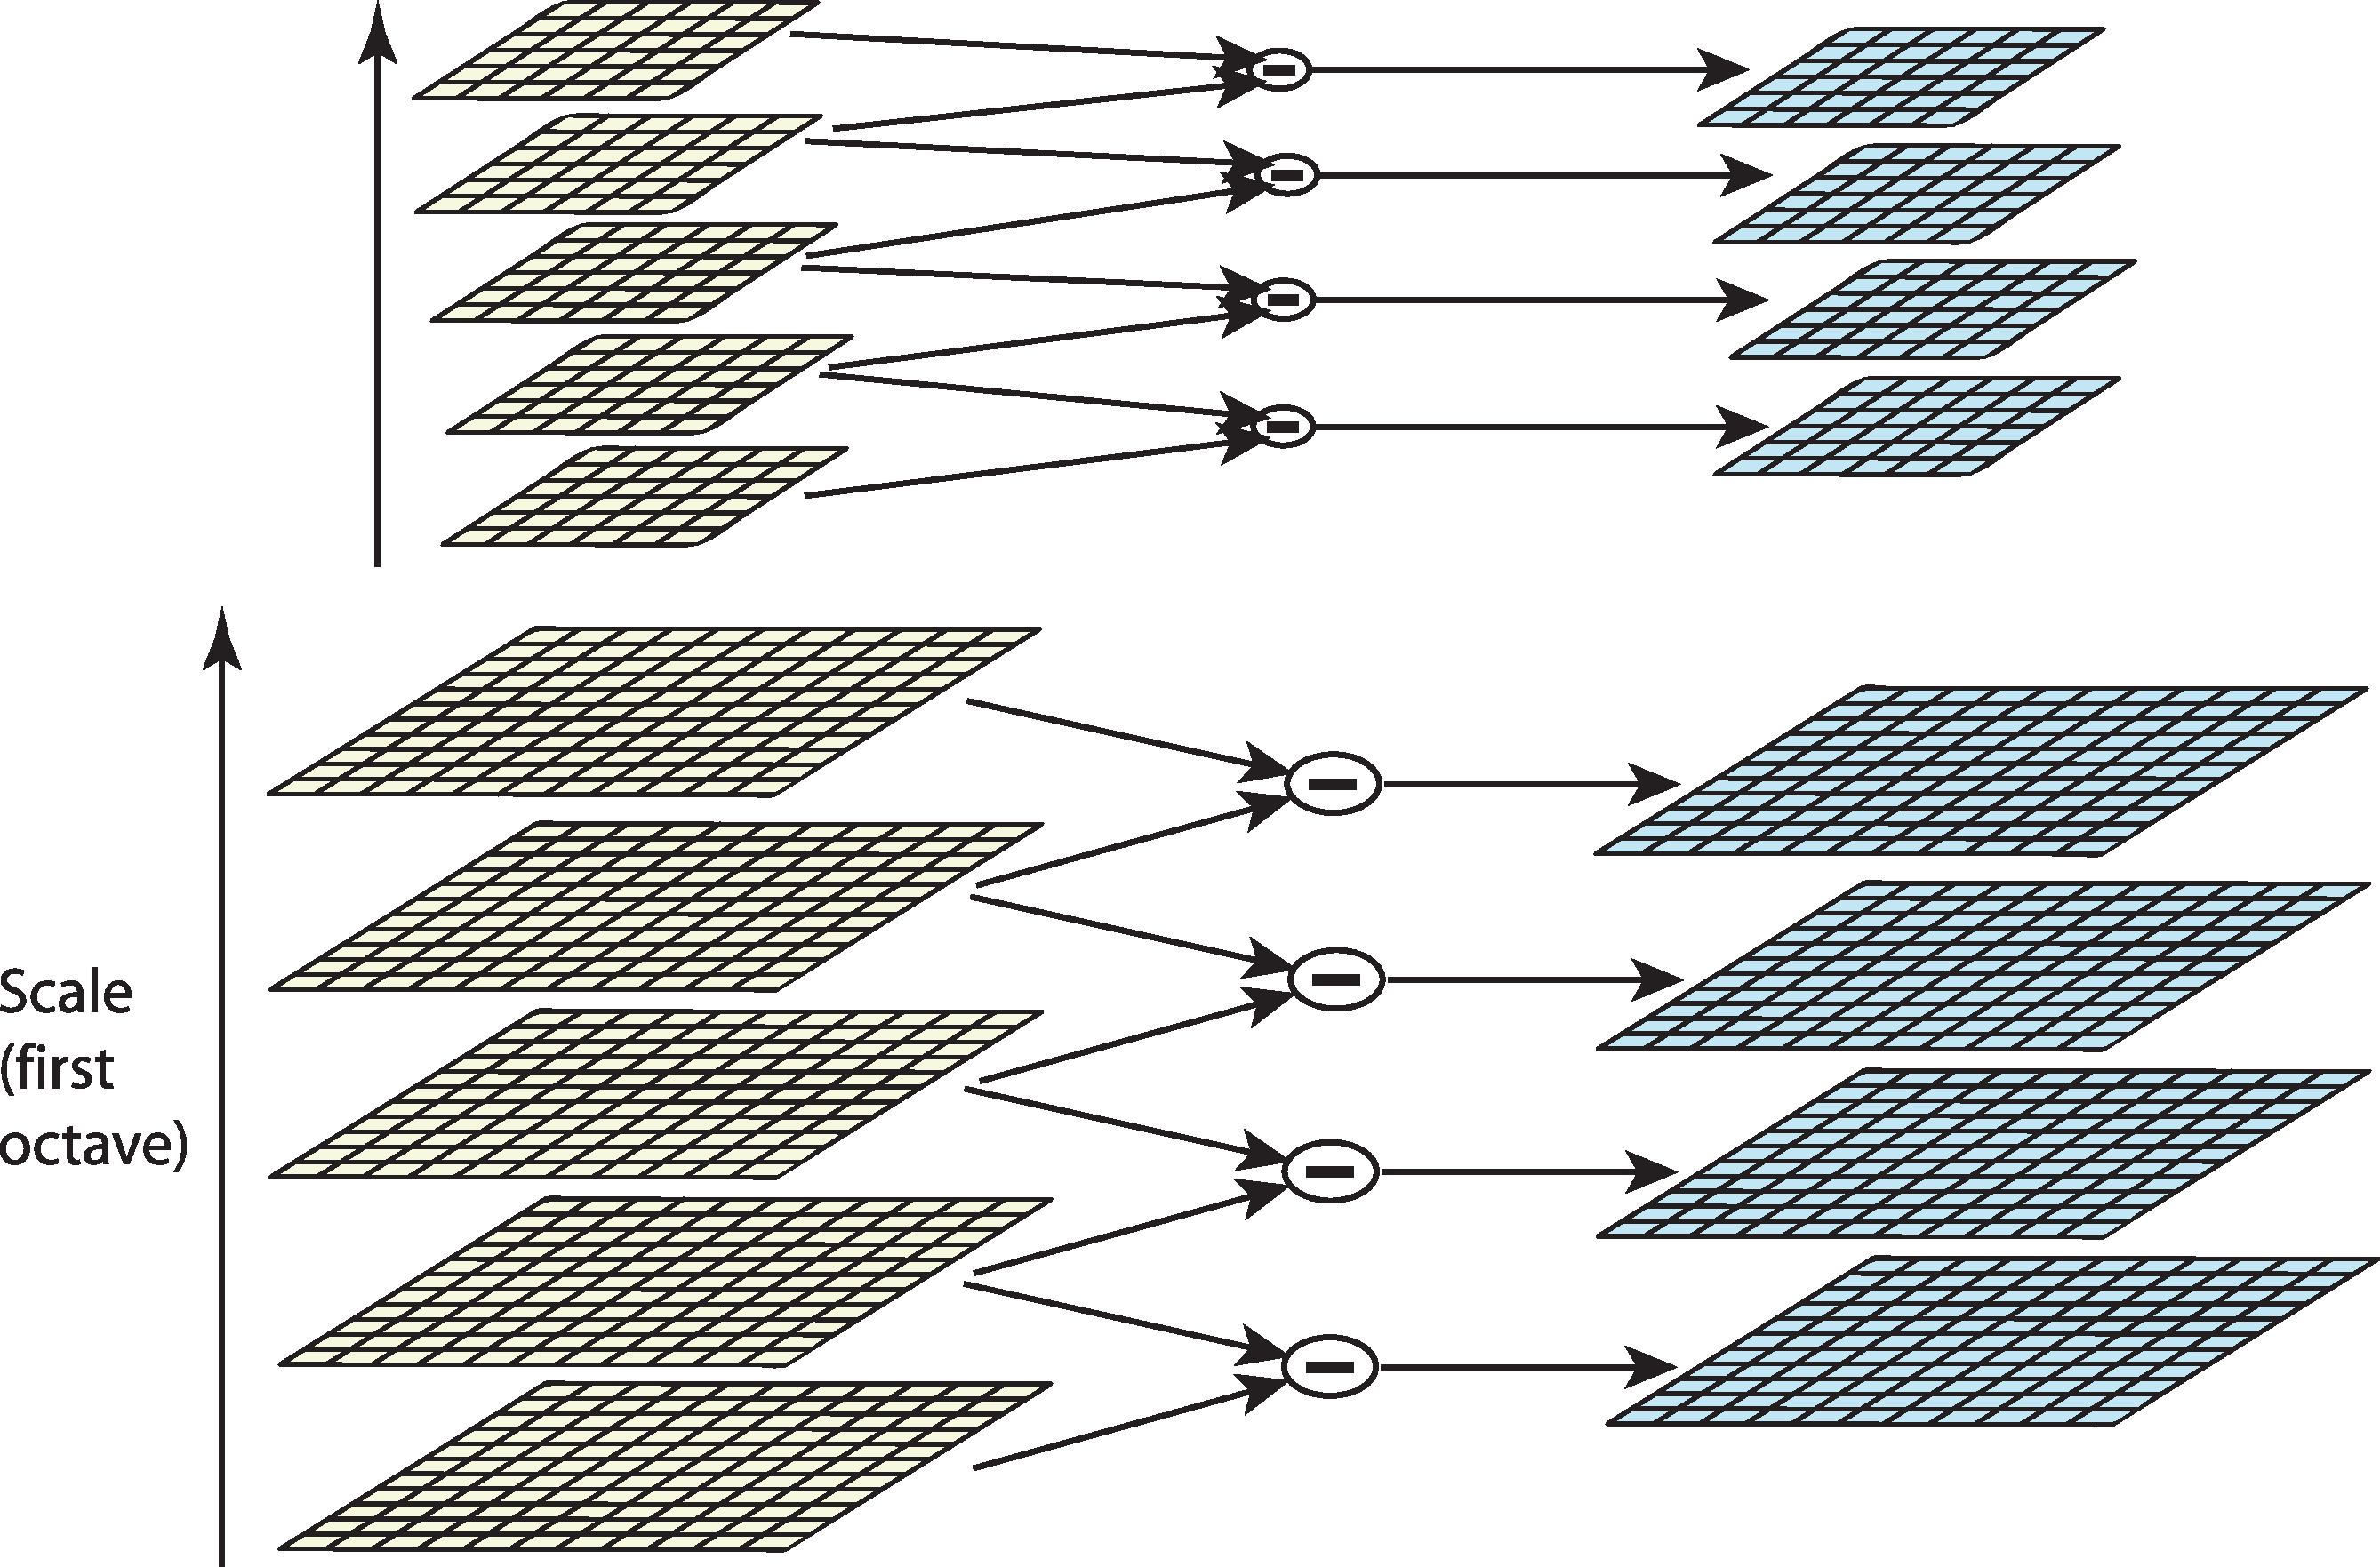
\includegraphics[width=1.0\textwidth,keepaspectratio]{Figures/sift_dog.pdf}
% \caption[Vizuální reprezentace výpočtu DoG v metodě SIFT]{Vizuální reprezentace výpočtu DoG v metodě SIFT. Převzato z \cite{sift}.}
% \label{fig:sift_dog}
% \end{figure}

Tato distinktivnost a robustnost SIFT deskriptorů umožňuje efektivní vyhledávání a párování klíčových bodů mezi obrázky, což je klíčové pro mnoho aplikací v oblasti počítačového vidění, jako je rozpoznávání scén a objektů či sledování pohybu. Díky těmto vlastnostem se SIFT stal základním stavebním kamenem pro mnohé následující výzkumy a aplikace v oblasti rozpoznávání obrazu \cite{sift}.

SIFT však není posledním vývojovým stupněm v technologiích detekce a popisu klíčových bodů. Od jeho vzniku bylo vyvinuto několik dalších algoritmů, které staví na jeho základech nebo se snaží překonat některé jeho omezení. Mezi tyto následující algoritmy patří například SURF (Speeded Up Robust Features) \cite{surf}, ORB (Oriented FAST and Rotated BRIEF) \cite{orb} a další, které se snaží zlepšit rychlost, efektivitu nebo invarianci k různým transformacím.
\endinput
\section{U-Net}
\label{sec:Chapter22}

\begin{figure}[ht]
\centering
\definecolor{boxcol}{rgb}{0.7,0.8,1.0}
\begin{tikzpicture}[
    box/.style={draw, inner sep=2pt, fill=boxcol, minimum height=30mm},
    skipbox/.style={draw, inner sep=2pt, fill=white, minimum height=30mm},
    rotate label/.style={anchor=south west, rotate=90, xshift=+0mm},
    redarrow/.style={->, draw=red, thick},
    grayarrow/.style={->, draw=gray, thick},
    bluearrow/.style={->, draw=blue, thick},
    greenarrow/.style={->, draw=green, thick},
    cyanarrow/.style={->, draw=cyan, thick}
  ]
  
  \coordinate (e00p) at (0,20); 
  \coordinate (e01p) at (0.75, 20);
  \coordinate (e02p) at (1.5, 20);
  
  \coordinate (e10p) at (1.5, 16.75);
  \coordinate (e11p) at (2.25, 16.75);
  \coordinate (e12p) at (3.0, 16.75);

  \coordinate (e20p) at (3, 14);
  \coordinate (e21p) at (4.25, 14);
  \coordinate (e22p) at (5.5, 14);

  \coordinate (b0p) at (5.5, 11.75);
  \coordinate (b1p) at (7.0, 11.75);
  \coordinate (b2p) at (8.5, 11.75);

  \coordinate (s0p)  at (7.79, 14);
  \coordinate (d00p) at (8.5,  14); 
  \coordinate (d01p) at (9.75, 14);
  \coordinate (d02p) at (11.0, 14);

  \coordinate (s1p)  at (10.57, 16.75);
  \coordinate (d10p) at (11.0, 16.75);
  \coordinate (d11p) at (12.0, 16.75);
  \coordinate (d12p) at (13.0, 16.75);

  \coordinate (s2p) at (12.78, 20);
  \coordinate (d20p) at (13.0, 20);
  \coordinate (d21p) at (13.75, 20);
  \coordinate (d22p) at (14.5, 20);
  \coordinate (d23p) at (15.25, 20);

  % Encoder
  \node[box, label=above:1, label={[rotate label]left:572x572}, inner sep=1pt] (e00) at (e00p) {};
  \node[box, label=above:64, label={[rotate label]left:570x570}] (e01) at (e01p) {};
  \node[box, label=above:64, label={[rotate label]left:568x568}] (e02) at (e02p) {};

  \node[box, label={[rotate label]left:$284^2$}, inner sep=2pt, minimum height=25mm] (e10) at (e10p) {};
  \node[box, label=above:128, label={[rotate label]left:$282^2$}, inner sep=4pt, minimum height=25mm] (e11) at (e11p) {};
  \node[box, label=above:128, label={[rotate label]left:$280^2$}, inner sep=4pt, minimum height=25mm] (e12) at (e12p) {};

  \node[box, label={[rotate label]left:$140^2$}, inner sep=4pt, minimum height=20mm] (e20) at (e20p) {};
  \node[box, label=above:256, label={[rotate label]left:$138^2$}, inner sep=8pt, minimum height=20mm] (e21) at (e21p) {};
  \node[box, label=above:256, label={[rotate label]left:$136^2$}, inner sep=8pt, minimum height=20mm] (e22) at (e22p) {};

  % Bottleneck
  \node[box, label={[rotate label]left:$68^2$}, inner sep=8pt, minimum height=15mm] (b0) at (b0p) {};
  \node[box, label=above:512, label={[rotate label]left:$66^2$}, inner sep=12pt, minimum height=15mm] (b1) at (b1p) {};
  \node[box, label={[rotate label]left:$64^2$}, inner sep=12pt, minimum height=15mm] (b2) at (b2p) {};

  % Decoder
  \node[skipbox, label=above:512, label={[rotate label]left:$128^2$}, inner sep=8pt, minimum height=20mm] (s0) at (s0p) {};
  \node[box, inner sep=12pt, minimum height=20mm] (d00) at (d00p) {};
  \node[box, label=above:256, label={[rotate label]left:$126^2$}, inner sep=8pt, minimum height=20mm] (d01) at (d01p) {};
  \node[box, label={[rotate label]left:$124^2$}, inner sep=8pt, minimum height=20mm] (d02) at (d02p) {};

  \node[skipbox, label=above:256, label={[rotate label]left:$248^2$}, inner sep=4pt, minimum height=25mm] (s1) at (s1p) {};
  \node[box, inner sep=8pt, minimum height=25mm] (d10) at (d10p) {};
  \node[box, label=above:128, label={[rotate label]left:$246^2$}, inner sep=4pt, minimum height=25mm] (d11) at (d11p) {};
  \node[box, label={[rotate label]left:$244^2$}, inner sep=4pt, minimum height=25mm] (d12) at (d12p) {};


  \node[skipbox, label={[rotate label]left:488x488}, inner sep=2pt, minimum height=30mm] (s2) at (s2p) {};
  \node[box, label=above:128, inner sep=4pt, minimum height=30mm] (d20) at (d20p) {};
  \node[box, label=above:64, label={[rotate label]left:486x486}, inner sep=2pt, minimum height=30mm] (d21) at (d21p) {};
  \node[box, label=above:64, label={[rotate label]left:484x484}, inner sep=2pt, minimum height=30mm] (d22) at (d22p) {};
  \node[box, label=above:2, label={[rotate label]left:484x484}, inner sep=1pt, minimum height=30mm] (d23) at (d23p) {};


  % Connect the boxes to form "U" shape
  \draw[bluearrow] (e00) -- (e01);
  \draw[bluearrow] (e01) -- (e02);
  \draw[redarrow] (e02) -- (e10);
  
  \draw[bluearrow] (e10) -- (e11);
  \draw[bluearrow] (e11) -- (e12);
  \draw[redarrow] (e12) -- (e20);
  
  \draw[bluearrow] (e20) -- (e21);
  \draw[bluearrow] (e21) -- (e22);
  \draw[redarrow] (e22) -- (b0);
  
  \draw[bluearrow] (b0) -- (b1);
  \draw[bluearrow] (b1) -- (b2);
  \draw[greenarrow] (b2) -- (d00);

  \draw[bluearrow] (d00) -- (d01);
  \draw[bluearrow] (d01) -- (d02);
  \draw[greenarrow] (d02) -- (d10);
  
  \draw[bluearrow] (d10) -- (d11);
  \draw[bluearrow] (d11) -- (d12);
  \draw[greenarrow] (d12) -- (d20);
  
  \draw[bluearrow] (d20) -- (d21);
  \draw[bluearrow] (d21) -- (d22);
  \draw[cyanarrow] (d22) -- (d23);

  \draw[grayarrow] (e02) -- (s2);
  \draw[grayarrow] (e12) -- (s1);
  \draw[grayarrow] (e22) -- (s0);


  \matrix [draw,below left, yshift=-0.5cm] at (current bounding box.south east) {
      \draw [bluearrow] (0,0) -- (0.5,0) node[right] {$3\times3$ Konvoluce + ReLU}; \\
      \draw [redarrow] (0,0) -- (0.5,0) node[right] {$2\times2$ Max Pooling}; \\
      \draw [grayarrow] (0,0) -- (0.5,0) node[right] {Propojení \& Oříznutí}; \\
      \draw [greenarrow] (0,0) -- (0.5,0) node[right] {$2\times2$ Up-sampling + $2\times2$ Konvoluce}; \\
      \draw [cyanarrow] (0,0) -- (0.5, 0) node[right] {$1\times1$ Konvoluce}; \\
  };
  
\end{tikzpicture}

\caption[Příkladná architektura sítě U-Net]{Architektura sítě U-Net s 3 bloky enkodéru a dekodéru. Vytvořeno podle \cite{unet}. }
\label{fig:unetdiagram}

\end{figure}

\textbf{U-Net} je architektura CNN poprvé představena v roce 2015 v literatuře \cite{unet}. Jedná se o architekturu konvoluční neuronové sítě hojně využívanou pro segmentační úlohy, avšak je používána i pro lokalizační, klasifikační a další problémy analýzy obrazu \cite{unet_success}. Architektura sítě U-Net spočívá ve třech sémantických částí, kde každá část zaznamenává jiné typy informací získaných z vstupních obrazů - enkodér, krk (ang. bottleneck) a dekodér. Závěrečná čtvrtá vrstva je specificky navržena a uzpůsobena pro konkrétní úkol, pro který je síť navržena.

\subsection{Stavba CNN sítě}
\label{subsec:Chapter221}

\textbf{Enkodér} sestává ze sémantických vrstev konvolučních bloků, kde každou sémantickou vrstvou sítě se zdvojnásobuje počet filtrů a rozměr obrazu se naopak dělí dvěma pomocí $2\times2$ max pooling vrstev na koncích bloků enkodéru. Cílem enkodéru je zachytit kontextuální rysy vstupního obrazu \cite{unet_success}.

\textbf{Krk (ang. bottleneck)} je prvek uprostřed sítě U-Net, která propojuje enkodér na jeho konci a dekodér na jeho počátku. Tato část sítě obsahuje nejmenší velikost obrazu, zato maximální počet filtrů v konvolučních vrstvách.

\textbf{Dekodér} je symetrická složka k enkodéru, kde každou sémantickou vrstvou sítě se počet filtrů naopak dělí dvěma. Vstup z předchozího bloku předchází $2\times2$ vrstva, v orig. lit. označená jako \enquote{up-convolution}. Ve skutečnosti se jedná o vrstvu $2\times2$ typu up-sampling následovanou $2\times2$ konvoluční vrstvou. Dekodér zachycuje vysoko-úrovňovější rysy a také je zodpovědný za finální lokalizaci \cite{unet_success}.

Všechny tyto 3 extrační části zpravidla obsahují dvě $3\times3$ konvoluční vrstvy. Původně v orig. lit. s odsazením typu valid padding a (1, 1) krokem (ang. stride). Mívají ReLU aktivační funkcí, obdobně jako v původní architektuře \cite{unet}. Postupem síť U-Net zlepšuje své receptivní pole, a v hlubších vrstvách se zlepšuje v zachycování sémantických a kontextuálních informací. Ovšem postupem síť také ztrácí lokalizační informace, pro které byly do sítě U-Net přidány také skokové propojení (tj. skip connection) mezi odpovídajícími vrstvami enkodéru a dekodéru \cite{unet_success}.

Těmito fundamentálními částmi sítě U-Net vzniká vizuální podoba písmena 'U', odkud pochází název sítě. Velikost sítě U-Net díky své symetrické a sémanticky jednoznačné architektuře může být zmenšena či zvětšena. Například v obrázku \ref{fig:unetdiagram} je síť sestavena ze 3 bloku enkodéru a dekodéru, avšak často se používá i velikost se 4 bloky (jako např. v originální literatuře \cite{unet}) nebo jiným počtem.

\subsection{Výstup CNN sítě}
\label{subsec:Chapter222}

Na konci sítě U-Net se nachází výstupní vrstva s několika filtry. Počet těchto filtrů odpovídá počtu tříd, které chceme v obrázku segmentovat. V případě binární segmentace (obdobně jako na obrázku \ref{fig:unetdiagram}), kde rozlišujeme mezi popředím a pozadím, se používají 2 filtry. Každý z těchto filtrů produkuje mapu pravděpodobností pro jednotlivé třídy.

Následně se aplikuje softmax funkce na výstupy těchto filtrů. Softmax je použit proto, aby se výstupy převedly na spojitou pravděpodobnostní distribuci, která umožňuje jednoznačně určit, zda pixel patří do popředí nebo pozadí. Softmax zajistí, že součet pravděpodobností pro každý pixel a pro všechny třídy bude roven 1, což umožňuje interpretovat výstupy jako pravděpodobnostní příslušnosti k jednotlivým třídám.

Je důležité poznamenat, že v případě více než dvou tříd segmentace se počet filtrů na konci U-Net odpovídajícím způsobem zvýší, aby každá třída měla svůj vlastní filtr. Následně se pro trénink sítí pro podobné segmentační úlohy, ať už binární nebo několika třídové, používají například ztrátové funkce z řad cross-entropy \cite{unet}.

\subsection{Využití}
\label{subsec:Chapter223}

U-Net se stal hojně používanou architekturou, kterou dnes můžeme nalézt i např. v biomedicínském inženýrství \cite{unet_success} nebo i difuzních modelech pro syntézi vysoko-rozměrových obrázků \cite{stablediffusion}.

Za rok 2022 se sítě U-Net oproti předchozím letům velmi rozšířily a např. v medicíně byly využity převážně pro segmentaci a klasifikaci. Avšak sítě U-Net byly schopny být aplikovány i na podobné problémy počítačového vidění, které zahrnují, ale neomezují se na rekonstrukce, detekce, deformační obrazová registrace\footnote{Problém mapovaní/transformace lehce deformovaného či posunutého obrazu na obraz druhý \cite{unet_registration}.}, odšumění či další. V roce 2022 dle zmíněné literatury bylo ocitováno téměř 3 tisíce vědeckých článků za rok, což je například trojnásobně vyšší počet než před dvěma lety v roce 2020 \cite{unet_success}.

\endinput
\section{U-Net++}
\label{sec:Chapter23}

Architektura U-Net++ byla představena v roce 2018 v literatuře \cite{unetpp} jako vylepšení původní architektury U-Net. Hypotézou této CNN architektury je zlepšení zachycení informací získaných v části enkodéru a následné obohacení o informace z hlubokých konvolučních bloků nahrazující plané skokové propojení původní sítě U-Net. Tyto obohacující konvoluční bloky byly přidány jako vyplnění sémantické trhliny ve skokových propojeních mezi enkodérem a dekodérem původní sítě U-Net. Přijímají také vstup ze všech předchozích bloků na stejné úrovni a výstup bloku z nižší vrstvy, na kterou je aplikována $2\times2$ vrstva typu up-sampling nebo transpose. Podoba sítě U-Net++ je zachycena na obrázku \ref{fig:unetpp} v části (a):

\begin{figure}[H]
\centering
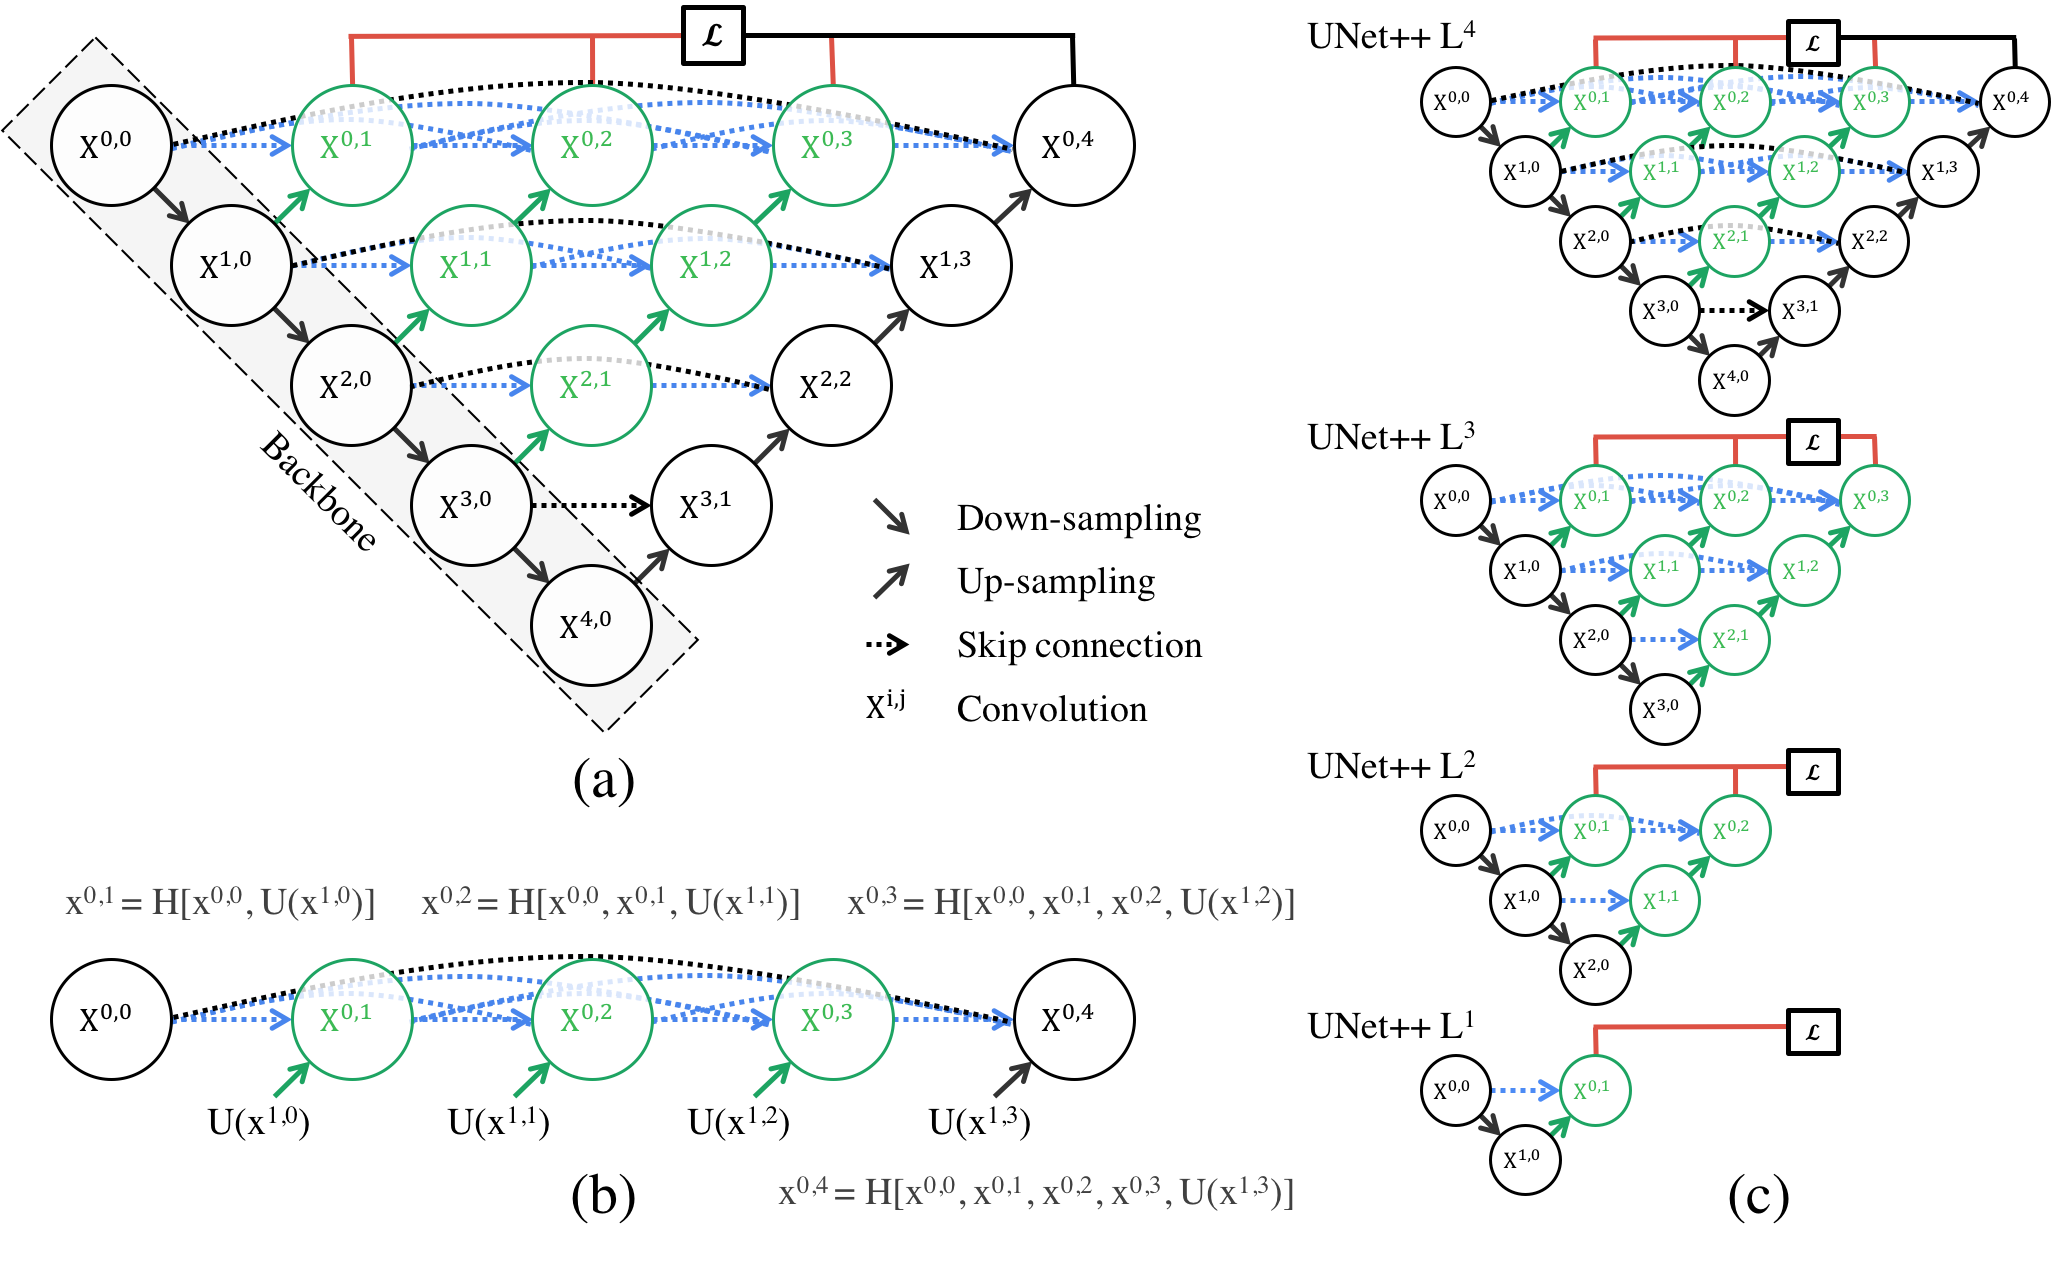
\includegraphics[width=1.0\textwidth,keepaspectratio]{Figures/unetpp.png}
\caption[Architektura sítě U-Net++]
{Architektura sítě U-Net++, kde je (a) obecný pohled na síť architektury U-Net++ s přidanými skokovými bloky a hlubokou supervizí \uppercase\expandafter{\romannumeral 50 \relax} (b) vrchní vrstva sítě U-Net mezi enkodérem a dekodérem, obsahující skokové bloky a jejich relevantní předcházející spoje (c) různé možnosti rychlého režimu modelu díky hluboké supervizi. Převzato z \cite{unetpp}. }
\label{fig:unetpp}
\end{figure}

U-Net++ představuje i druhou změnu -- možnost \textbf{hluboké supervize}. Pokud byla síť trénována v módu hluboké supervize, pak hluboká supervize nám dovoluje využívat model při inferenci v jednom ze dvou režimů:

\begin{enumerate}
    \item \textbf{Přesný režim}, kde se využívají všechny bloky v blocích \{\(x^{0, j} \colon j \in \{1,2,...,n\}\)\}, kde \(n\) tvoří počet bloků v první (nejméně hluboké) vrstvě konvolučních bloků propojující enkodér-dekodér sítě U-Net++ \cite{unetpp}. V tomto režimu využíváme všechny pomocné výstupy těchto bloků, kde výstupní mapa příznaků tvoří průměr map příznaků těchto výstupů.
    \item \textbf{Rychlý režim}, kde použijeme tzv. pruning (vyobrazen na obrázku \ref{fig:unetpp} v části c) pro snížení velikosti (a tedy i parametrů) sítě, kde výslednou mapu tvoří poslední konvoluční blok v první vrstvě vnořených bloků sítě U-Net++. Síť v tomto režimu dokáže pracovat rychleji, zato méně přesněji.
\end{enumerate}

Samozřejmě pro každý použitý výstup se aplikuje relevantní výstupní vrstva, např. $1\times1\times1$ konvoluční vrstva s aktivační funkci sigmoid.

\endinput
\section{Attention U-Net}
\label{sec:Chapter24}

Vylepšení sítě U-Net o \textbf{pozornostní bloky} či brány (AG, tj. attention gates) bylo představeno v literatuře \cite{attentionunet} roku 2018. Základní myšlenkou pozornostních bloků je umožnit síti lépe se soustředit na relevantní části vstupního obrazu a současně se naučit ignorovat irelevantní části. Vylepšení pozornostních bloků bylo přidáno do části dekodéru sítě U-Net. Pozornostní bloky přijímají 2 vstupy, kde jeden z nich je bránový vstup $g$ z předchozího bloku a druhý je skokové propojení z odpovídající vrstvy enkodéru $x^l$. Pozornostní blok je detailněji ilustrován na obrázku \ref{fig:attention_unet}:

\begin{figure}[H]
\centering
\definecolor{boxcol}{rgb}{0.7,0.8,1.0}
\begin{tikzpicture}[
    box/.style={draw, thick, minimum width=2cm, minimum height=0.75cm, text centered, fill=boxcol, text width=2.1cm},
    activation/.style={draw, thick, minimum width=1.6cm, minimum height=0.75cm, text centered, fill=white, text width=1.6cm},
    arrow/.style={->, thick},
    resampler/.style={
        matrix of nodes,
        nodes in empty cells,
        nodes={draw, minimum size=5mm, inner sep=0pt, outer sep=0pt, fill=gray!30},
        column sep=-\pgflinewidth,
        row sep=-\pgflinewidth,
        fill=white,
    },
    shortarrow/.style={->, shorten >=0.35cm},
]
  \coordinate (wgp) at (0,4);
  \coordinate (wxp) at (0,2);
  \coordinate (plusp) at (2, 3);

  \coordinate (relup) at (4, 3);
  \coordinate (psip) at (6.75, 3);
  \coordinate (sigmoidp) at (9.5, 3);

  \coordinate (resamplerp) at (11.75, 3);
  \coordinate (timesp) at (13.5, 3);

  \node[box] (wg) at (wgp) {$W_g \colon 1\times1\times1$};
  \draw [arrow] ([xshift=-0.75cm]wg.west) -- (wg.west) node [midway, above] {$g$};
  \node[below=of wg, yshift=1.0cm] {$F_g \times H_g \times W_g \times D_g$};

  \node[box] (wx) at (wxp) {$W_x \colon 1\times1\times1$};
  \draw [arrow] ([xshift=-0.75cm]wx.west) -- (wx.west) node [midway, above] {$x^l$};
  \node[below=of wx, yshift=1.0cm] {$F_l \times H_x \times W_x \times D_x$};

    % koordinát pro vlevo od boxíku
  \coordinate (xlbranchp) at ([xshift=-0.55cm, yshift=-0.025cm]wx.west);
  \coordinate (xlbranch_inter_p) at ([yshift=-3cm, xshift=-1.75cm]wg.south);

  \node (plus) at (plusp) {{\Huge $\oplus$}};
  \draw [arrow] (wg) -| (plus);
  \draw [arrow] (wx) -| (plus);

  \node[activation] (relu) at (relup) {ReLU};
  \draw[arrow] (plus) -- (relu);
  \node[below=of relu, yshift=1.00cm, xshift=0.1cm] {$F_{int} \times H_g \times W_g \times D_g$};
  
  \node[box] (psi) at (psip) {$\psi \colon 1\times1\times1$};
  \draw[arrow] (relu) -- (psi);
  
  \node[activation] (sigmoid) at (sigmoidp) {Sigmoid};
  \draw[arrow] (psi) -- (sigmoid);
  \node[below=of sigmoid, yshift=1.00cm, xshift=-1.2cm] {$H_g \times W_g \times D_g$};

  \matrix (resampler) [resampler] at (resamplerp) {
    {} & {} & {} \\
    {} & {} & {} \\
    {} & {} & {} \\
  };
  \node[above=of resampler, yshift=-1.0cm] {Převzorkovník};
  \node[below=of resampler, yshift=1.0cm, xshift=0.4cm] {$H_x \times W_x \times D_x$};
  
  \draw[arrow] (sigmoid) -- (resampler);

  \node (times) at (timesp) {{\Huge $\otimes$}};
  \draw [->] (times.east) -- ++(0.5cm,0) node [midway, above] {$\hat{x}^l$};
  \draw[shortarrow] (resampler) -- (timesp) node[midway, above, xshift=-0.25cm] {$\alpha$};
  \draw[arrow] (xlbranchp) -| (xlbranch_inter_p) -| (times);
\end{tikzpicture}
\caption[Pozornostní blok sítě Attention U-Net]{Pozornostní blok sítě Attention U-Net, kde $g$ je bránový vstup, $x^l$ je vstup ze skokového propojení, $\psi$ je konvoluční operace s trénovatelnými parametry. $\hat{x}^l$ je finálně výsledek vzájemného součinu pozornostních koeficientů $\alpha$ a $x^l$. Vytvořeno podle \cite{attentionunet}. }
\label{fig:attention_unet}
\end{figure}

Aby byla zajištěna kompatibilita, jsou rozměry bránového signálu $g$ a skokového propojení z výstupu relevantního bloku enkodéru $x^l$ přizpůsobeny na rozměry bránového signálu $H_g \times W_g \times D_g$. Prvky jsou po aplikaci oddělených konvolucích sečteny na elementární úrovni a následně použity jako vstup do konvolučních vrstev ReLU a sigmoid. Konvoluční vrstva s aplikační funkcí sigmoid generuje koeficienty pozornosti ($\alpha_i$).

Mechanismus pozornosti funguje tak, že se na kombinované rysy aplikuje aktivace sigmoid pro generování koeficientů pozornosti (\(\alpha_i\), kde \(\alpha_i \in (0, 1)\)), které účinně škálují vstupní rysy tím, že zvýrazňují oblasti zájmu a potlačují méně relevantní oblasti. Tohoto selektivního zvýraznění je dosaženo prostřednictvím elementárního násobení koeficientů pozornosti s rysy vstupu $x^l$, což zajišťuje, že se síť zaměřuje na relevantní informace z první části sítě. Toto tvoří výstup pozornostních bloků \cite{attentionunet}.

\endinput
\section{ResUNet-a}
\label{sec:Chapter25}

ResUNet-a je bohaté rozšířeni původní sítě U-Net o hned několik změn, poprvé představeno v \cite{resuneta} roku 2019. Síť je obohacena o \textbf{reziduální bloky} (představeny v \cite{residualblocks}), \textbf{dilatované konvoluce}, \textbf{PSP pooling} (představen v \cite{psp}) vrstvy a \textbf{multi-taskové učení}. Síť je také v této literatuře trénována na své adaptaci Diceovy loss funkce. Vysoko-úrovňová podoba sítě je představena na obrázku \ref{fig:resuneta_overview}.

\textbf{Reziduální bloky} jsou zde použity namísto klasických bloků U-Net jak v enkodéru, tak v dekodéru původní architektury U-Net. Slouží pro adresování problému explodujících či ztrácejících se gradientů při fázi učení hlubokých sítí. Do reziduálních bloků jsou také přidány dilatované konvoluce, které zvyšují receptivní pole bez navýšení parametrů sítě. Hodnoty dilatací jsou ve vrstvách rozděleny různě pro zachycení několika velikostí receptivního pole. Vrstvy vně reziduálních bloků sdílí stejný počet filtrů, počet filtrů v bloku se samozřejmě hloubkou enkodéru zdvojnásobuje a dekodéru dělí dvěma, jako v původní síti U-Net.

Vrstvy typu \textbf{PSP pooling} (Pyramid Scheme Parsing) se nacházejí namísto krku sítě a před 1x1 konvoluční vrstvou pro finální segmentaci sítě ResUNet-a (viděných na obrázku \ref{fig:resuneta_overview}). Tyto bloky slouží pro zachycení kontextuálních informací na různých škálách. Vstupní mapy příznaků (ang. feature maps) jsou v několika větvích různě zmenšeny v rozměrech a následně opět zvětšeny do původní velikosti. Tyto větvě jsou následně spojeny do společného výstupu na ose filtrů. Je nutno podotknout, že PSP bloky jsou také konstruovány reziduálně.

\begin{figure}[H]
\centering
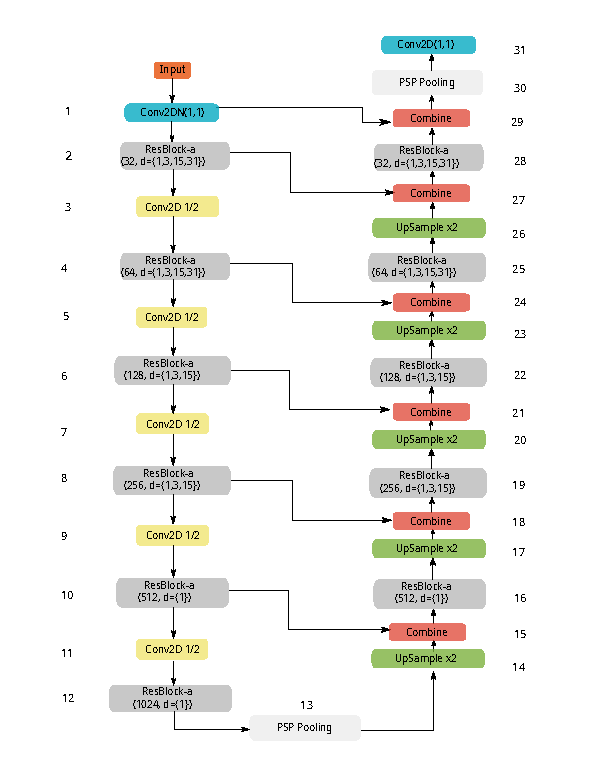
\includegraphics[width=0.7\textwidth,keepaspectratio]{Figures/resuneta_overview.pdf}
\caption[Obecný přehled architektury ResUNet-a]{Obecný přehled architektury ResUNet-a bez použití multi-taskového učení. Převzato z \cite{resuneta}. }
\label{fig:resuneta_overview}
\end{figure}

\textbf{Multi-taskové učení} představeno v originální literatuře slouží ke zlepšení výsledků segmentační úlohy. Při aplikaci multi-taskového učení se nahradí finální 1x1 konvoluční vrstva, PSP pooling vrstva a kombinační vrstva na výstupu jednodušší sítě ResUNet-a. Pro segmentační úlohu jsou si všechny 4 části na sobě komplementární a na sobě nezávisle vygenerovány. Je nutno podotknout, že tyto části nejsou určeny pro přímou součástí finálních inferenčních výsledků, avšak pro vylepšení generalizační a sémanticky chápající schopnosti sítě během tréninku. Učením těchto doplňkových úloh získává síť další informace, které nepřímo přispívají ke zlepšení přesnosti a kvality primární úlohy: segmentace. Konkrétně se jedná o následující 4 části: \cite{resuneta}: 
\begin{enumerate}
    \item Segmentační masky
    \item Hranové masky, pro zlepšení pochopení rozsahu segmentační úlohy
    \item Vzdálenostní masky, zlepšující \enquote{propojení} topologického uspořádání mezi třídami na obrazu, jako je např. mezi autem a cestou na které stojí. V orig. lit. zmíněno např. segmentační maska pro cestu s "dírou" v místě, kde má být auto. Oba tyto objekty zároveň panují jako vlastní třídy součástí sítě.
    \item Výstupu obrázku v barevném modelu HSV
\end{enumerate}
\endinput
\section{YOLOv8}
\label{sec:Chapter26}
YOLOv8 je jeden z posledních state-of-art přístupů pro lokalizaci, klasifikaci, segmentaci, detekci a dokonce také i tracking objektů představených v roce 2023 firmou Ultralytics. V době psaní tohoto textu je dostupná již i verze 8.1. Rodina skupiny YOLO, která je v poslední době velmi populární, se vyznačuje svou rychlostí a přesností, což ji udělalo skvělou volbou pro analýzu obrazu pomocí hlubokého učení. Každá verze se snažila vylepšit nedostatky nebo zlepšit ostatní parametry svých předchůdců. YOLOv8 (včetně jeho vylepšení jako verze 8.1) je v současné době poslední verzí a nebyl vydán oficiální papír dokumentující vývoj a metodické představení, avšak uchytil se již například v \cite{yoloplane} pro detekci a klasifikaci letadel či dronů. Existuje hned několik velikostí tohoto modelu:
\begin{enumerate}
  \item YOLOv8n -- nejmenší (nano), 3.2 M parametrů
  \item YOLOv8s -- malý (small), 11.2 M parametrů
  \item YOLOv8m -- střední (medium), 25.9 M parametrů
  \item YOLOv8l -- velký (large), 43.7 M parametrů
  \item YOLOv8xl -- extra velký (extra large), 68.2 M parametrů
\end{enumerate}

YOLOv8 je nejlépe srovnatelná s předchůdcem YOLOv5, který byl také vydaný stejnojmennou firmou (stejně také i verzi 1 či 3). Používá Darknet53 \cite{darknet} jako základ pro svou první část své architektury s několika změnami. Darknet53 se vyznačuje reziduálními bloky a malými velikostmi filtrů. Další části jsou krk a hlava. Krk propojuje základ a hlavu zlepšující zachycení informací na různých škálách. Hlava je finální část a ve verzi 8 je oddělená pro zpracování dané úlohy separátně pro každou úlohu. Verze 8 také navazuje na trend posledních let nemívat kotvy ve své architektuře, což jsou boxy s předdefinovaou velikostí sloužící k prototypové detekci objektů \cite{yolo_comparison}.


\endinput
\section{DINOv2}
\label{sec:Chapter27}

DINOv2 je dalším z state-of-art přístupů představených v \cite{dinov2} roku 2023. Jedná se o model pod vlastním dohledem schopný dosáhnout řešit mnoho problémů počítačového vidění. Páteřní síť DINOv2 je síť s pomocí ViT pozornostních visuálních bloků (ang. Vision Transformer) \cite{vit}. Hlavní předtrénovaný model obsahuje přes 1 miliardu parametrů.

Model DINOv2 nachází uplatnění v řadě pokročilých úloh zpracování obrazu. Jeho využití je rozmanité a zahrnuje techniky jako segmentaci a klasifikaci, ale dokonce i odhad hloubky, párování typu dense matching nebo párování mezi sémanticky odpovídajícími klíčovými body (ang. sparse matching), vyobrazeno na obrázku \ref{fig:dinov2_sparse_matching}. Oba typy párování nachází relevantní části obrázku mezi sémanticky podobnými scénámi \cite{dinov2.metademolab.com}.

\begin{figure}[H]
\centering

\newcommand{\subfiguresize}{.15\textwidth}
\newcommand{\imagewidth}{1.0in}
\newcommand{\hspacesize}{.43in}

\newcommand{\insertimage}[1]{%
  \begin{minipage}{\imagewidth}
    \centering
    \includegraphics[width=\imagewidth]{#1}
  \end{minipage}
}

\subfloat[Ptáci / Letadla]{%
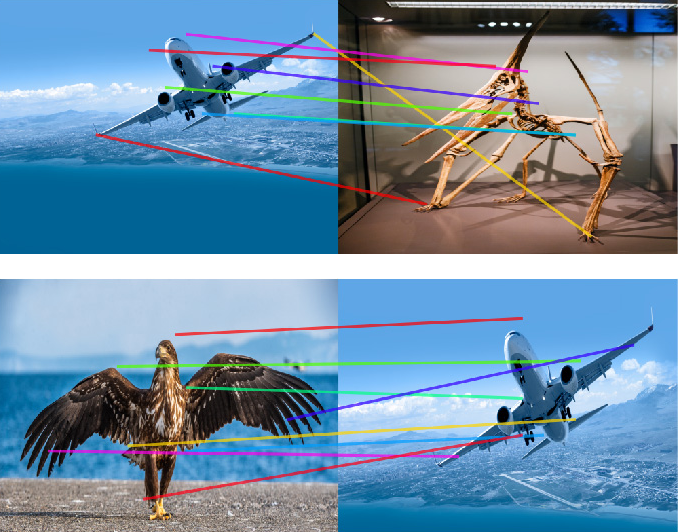
\includegraphics[width=0.4\textwidth,keepaspectratio]{Figures/dinov2_sparse_half_1.png}
  \label{fig:dinov2_birds_airplanes}%
}\hspace{\hspacesize}%
\subfloat[Vozidla]{%
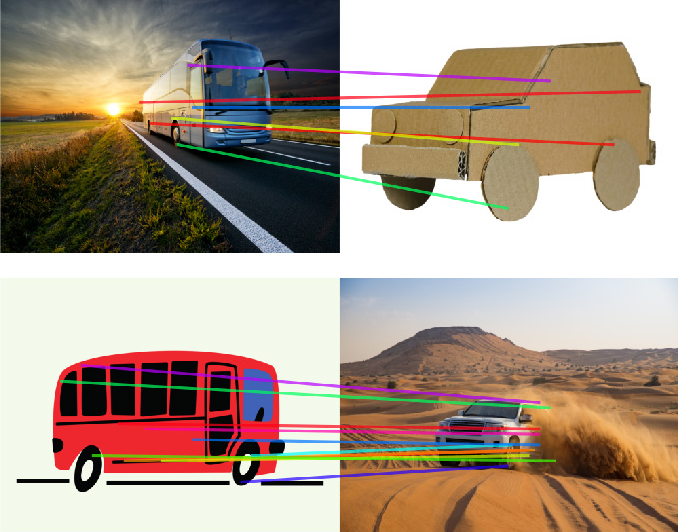
\includegraphics[width=0.4\textwidth,keepaspectratio]{Figures/dinov2_sparse_half_2.png}
  \label{fig:dinov2_vehicles}%
}

\caption[Využití DINOv2 pro párování typu sparse matching]
{Využití DINOv2 pro párování typu sparse matching mezi sémanticky podobnými scénami. Převzato z \cite{dinov2} a přeloženo.}
\label{fig:dinov2_sparse_matching}
\end{figure}

\endinput
\section{Transformer STN}
\label{sec:Chapter28}

Architektura STN je jedním z možných přístupů, jak představit prostorovou invarianci do klasických konvolučních neuronových sítí. Byla představena v literatuře \cite{stn} roku 2015. Klasické konvoluční neuronové sítě pomocí svých vrstev typu max pooling\footnote{v síti U-Net nacházející se v enkodéru.} tvoří jistou prostorovou invarianci proti různým změnám perspektivy, avšak pouze limitovaně. Výrazné transformace vstupního obrazu mívají detrimentální účinek na výslednou robustnost sítě.

Pro řešení této limitace týkající se prostorové invariance vznikla neuronová síť s prostorovým transformerem -- \textbf{STN (ang. Spatial Transformer Network)}. Z původního hlediska se často nejedná o hotové řešení, avšak o diferenciovatelný modul schopný být přidán do již existující architektury konvolučních neuronových sítí pro zvýšení odolnosti proti těmto prostorovým změnám a transformacím. Oproti klasickým vrstvám typu max pooling je tato síť schopna se naučit a aktivně transformovat vstupní obraz. Modul také díky své diferenciovatelnosti může být triviálně natrénován pomocí klasické zpětné propagace. Modul STN sestává z několika částí (viděných na obrázku \ref{fig:stn_overview}):

\begin{figure}[ht]
\centering
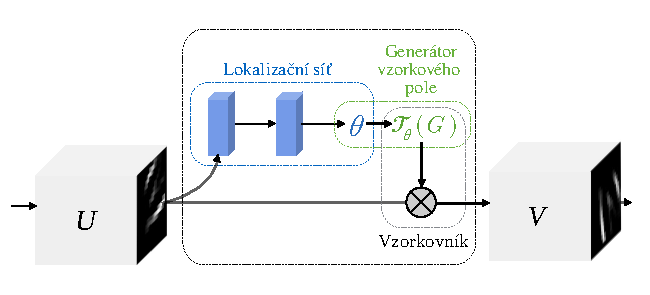
\includegraphics[width=0.8\textwidth,keepaspectratio]{Figures/stn/stn_module.pdf}
\caption[Zjednodušený pohled na STN modul]
{Zjednodušený pohled na STN modul, kde $U$ je vstupní obraz a $V$ je výstupní obraz. Lokalizační síť provádí regresi transformačních parametrů $\theta$, která je pak využita pro generování vzorkového pole. Příkladná vizualizace vzorkového pole, a jeho použití ve vzorkovníku, je znázorněna na obrázku \ref{fig:stn_grid}. Převzato z \cite{stn} a upraveno. }
\label{fig:stn_overview}
\end{figure}

\subsection{Lokalizační síť}

První částí je \textbf{lokalizační síť} (ang. localization net). Právě tato část modulu je jako jediná trénovatelná. Vstupem do lokalizační sítě může být jakýkoli n-kanálový obraz či mapa příznaků. Výstup lokalizační sítě jsou parametry $\theta$ společné pro všechny kanály vstupního snímku. Architektura sítě není striktně dána, může být postavena jak na CNN nebo FCN za předpokladu, že finální část sítě bude uzpůsobena pro regresi parametrů afinní transformace $\theta$ reprezentovanou v matici ${\displaystyle \mathrm {A} }_\theta$.

Matice ${\displaystyle \mathrm {A} }_\theta$ může nabývat několika forem. Prvním klasickým přístupem může být následující matice $2\times3$:
\begin{equation}
    {\displaystyle \mathrm {A} }_\theta = 
    \begin{bmatrix}
        \theta_{11} & \theta_{12} & \theta_{13} \\
        \theta_{21} & \theta_{22} & \theta_{23}
    \end{bmatrix}
    \label{eq:stn_6_theta}
\end{equation}
pro translaci, rotaci, škálování a zkosení podél os. Matice ${\displaystyle \mathrm {A} }_\theta$ avšak může nabývat i více podob, jako např. 12člennou matici $4\times3$ pro 3D afinní transformace nebo následující poupravenou afinní 2D matici pro prostorovou pozornost, umožňující translaci, izotropní škálování a ořezávání:

\begin{equation}
    {\displaystyle \mathrm {A} }_\theta = 
    \begin{bmatrix}
        s & 0 & t_x \\
        0 & s & t_y
    \end{bmatrix}.
    \label{eq:stn_3_theta}
\end{equation}

Ořezávání je dosaženo s pomocí levé $2\times2$ strany matice ${\displaystyle \mathrm {A} }_\theta$ zapsanou jako ${\displaystyle \mathrm {A'} }_\theta$. Pokud platí, že $determinant({\displaystyle \mathrm {A'} }_\theta) < 1$, pak je výsledná plocha transformace menší než plocha originálního vstupu a vzorkové pole se soustředí pouze na jistou část snímku, což vede k lokálnější prostorové pozornosti.

\subsection{Generátor vzorkového pole}

Výstup lokalizační sítě, matice ${\displaystyle \mathrm {A} }_\theta$, pak následuje do další části modulu STN -- \textbf{generátoru vzorkového pole} (v originální ang. podobě grid generator). Generátor vzorkového pole generuje dvousložkové pole, které aplikuje parametry afinní transformace ${\displaystyle \mathrm {A} }_\theta$. K tomu se využívá způsob inverzního mapování.

\begin{figure}[h]
\centering
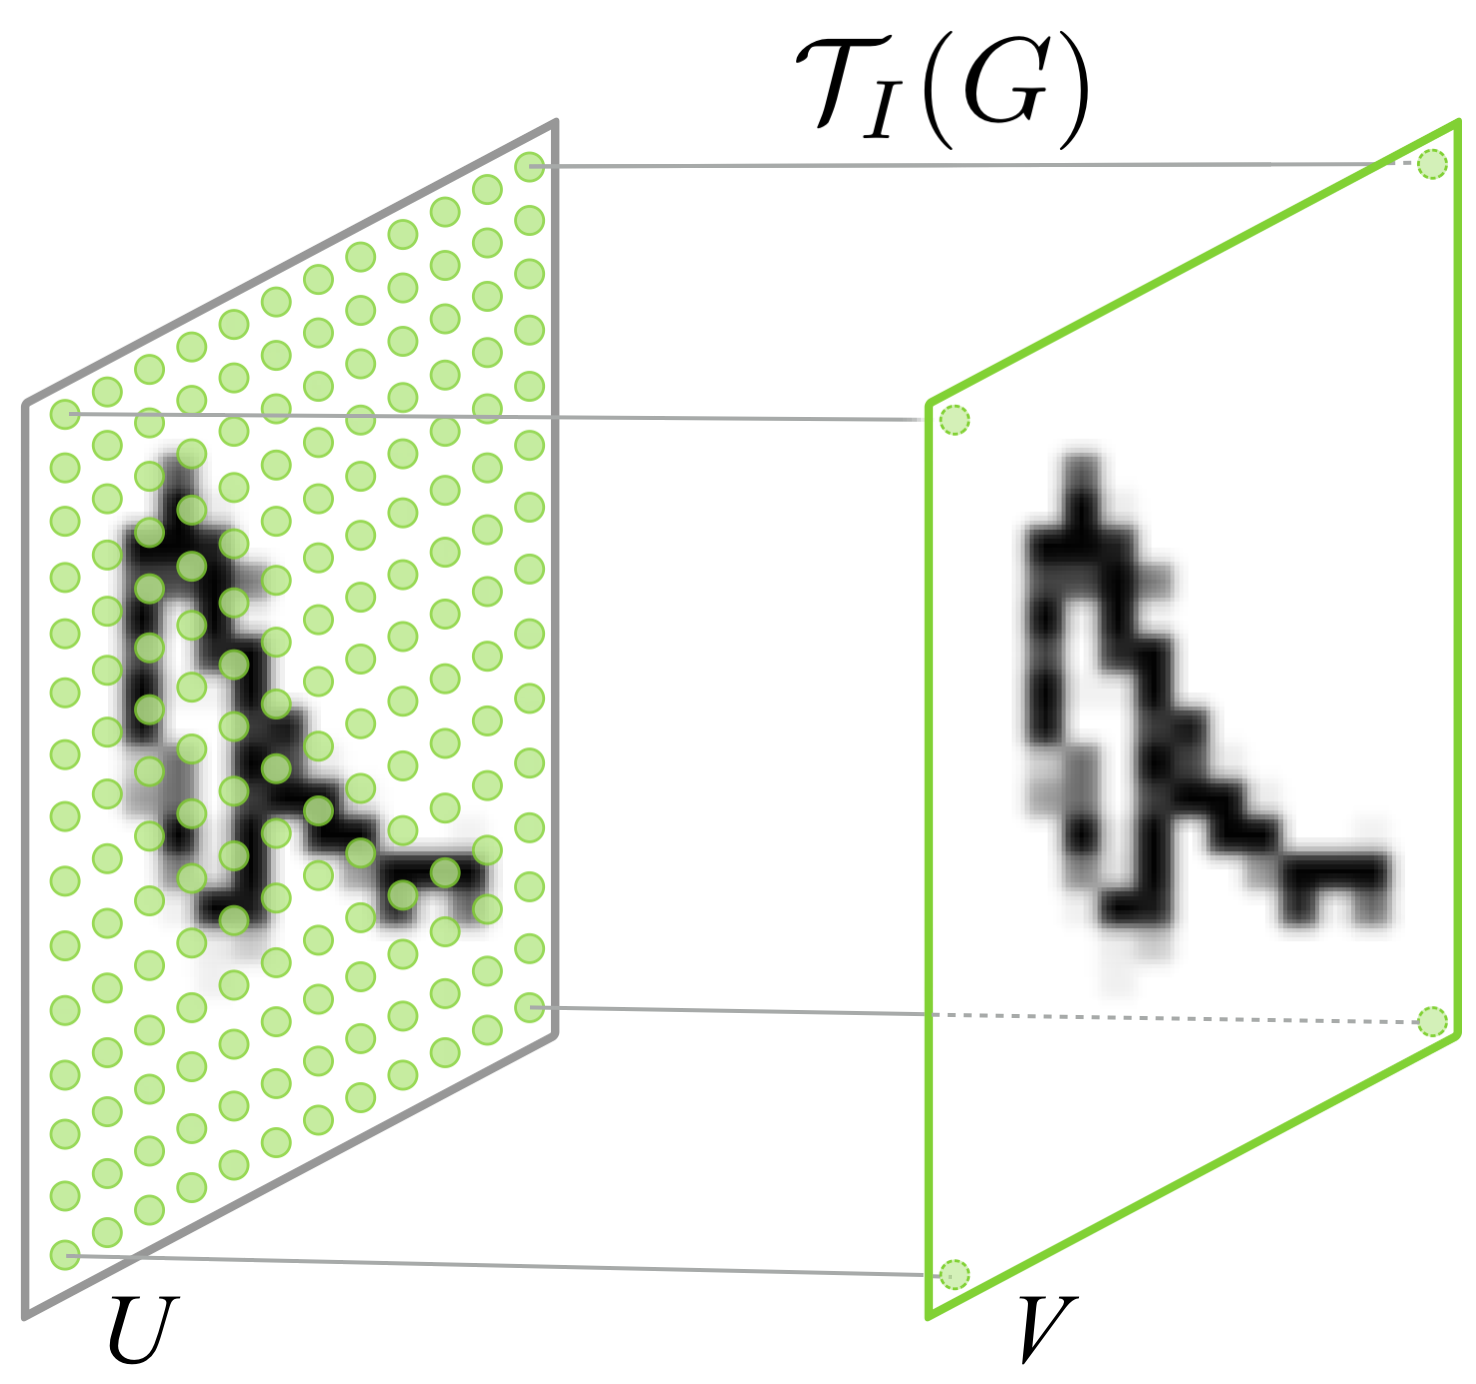
\includegraphics[width=0.3\textwidth,keepaspectratio]{Figures/stn/stn_a.png}
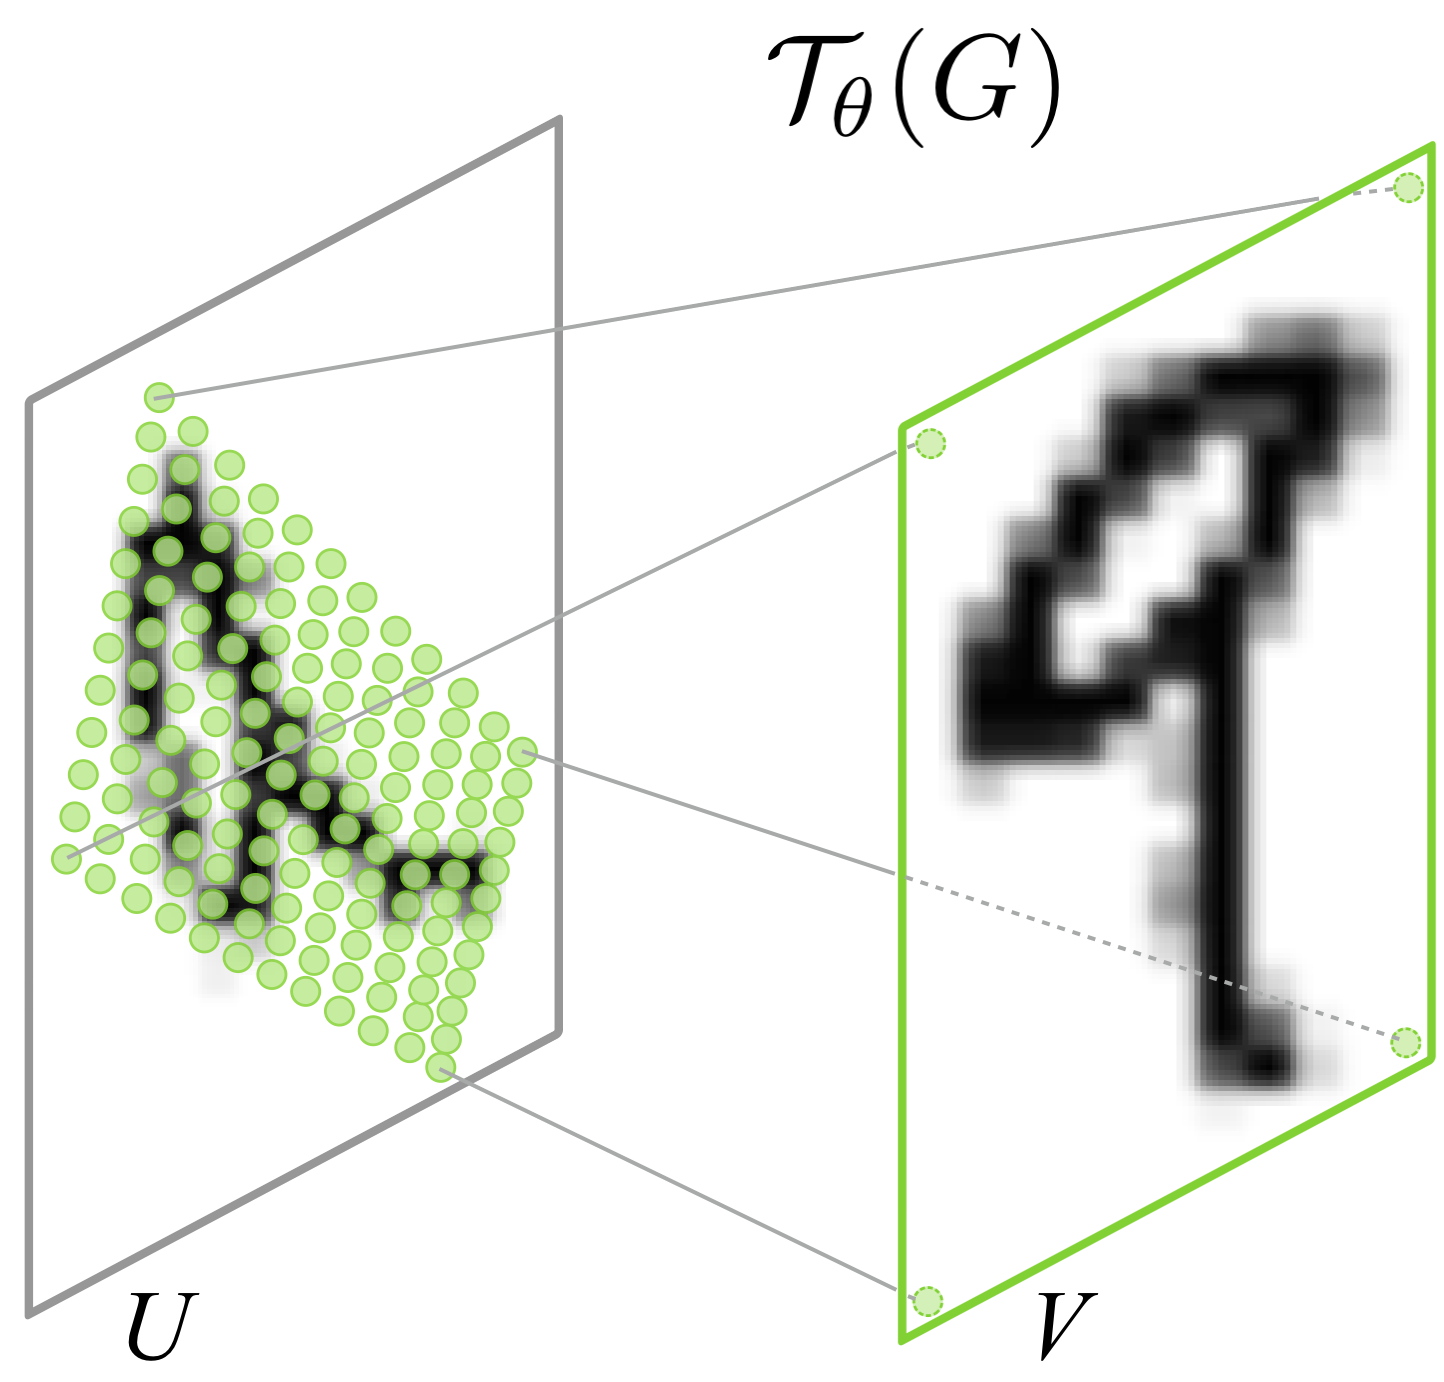
\includegraphics[width=0.3\textwidth,keepaspectratio]{Figures/stn/stn_b.png}
\caption[Vizualizace generování vzorkového pole v modulu STN]
{Vizualizace generování vzorkového pole v modulu STN a jeho aplikace na transformování vstupního snímku ve vzorkovníku, kde $T_{\theta}(G)$ je 2D skalární pole s transformovanými souřadnicemi pravidelné mřížky (ang. regular grid) $G$ zdrojového pole. $T_{I}(G)$ je jednotková transformace. Převzato z \cite{stn}. }
\label{fig:stn_grid}
\end{figure}

Inverzní mapování je často použito oproti přímému mapování, jenž nefunguje dobře díky přesahům a mezerám, které zanechá při mapování ve výsledném snímku. Inverzní mapování bývá standardním postupem v praxi při podobných úlohách počítačového vidění \cite{stn_medium_1}. Inverzní mapování v kontextu STN ve 2D prostoru může být (identicky jako v originální literatuře \cite{stn}) definováno takto:

\begin{equation}
\begin{pmatrix}
x_i^s \\
y_i^s
\end{pmatrix}
= T_{\theta}(G_i) = {\displaystyle \mathrm {A} }_\theta
\begin{pmatrix}
x_i^t \\
y_i^t \\
1
\end{pmatrix}
= 
\begin{bmatrix}
\theta_{11} & \theta_{12} & \theta_{13} \\
\theta_{21} & \theta_{22} & \theta_{23}
\end{bmatrix}
\begin{pmatrix}
x_i^t \\
y_i^t \\
1
\end{pmatrix},
\label{eq:stn_inverse}
\end{equation}
kde $(x_i^s, y_i^s)$ je daná pozice na původním obrazu, kterou počítáme pomocí funkce inverzního mapování na základě transformovaného vzorkového pole $T_{\theta}(G)$. To lze vyjádřit jako násobení matice ${\displaystyle \mathrm {A} }_\theta$ a cílové pozice v homogenní formě $(x_i^t, y_i^t, 1)$. Výsledkem použití inverzního mapování (ve funkci \ref{eq:stn_inverse}) je vzorkové pole reprezentované také jako 2D dvousložkové pole či dvě 2D skalární pole pro osy $(x, y)$.

\subsection{Vzorkovník}

Pro provedení prostorové transformace na originálním snímku modulu STN zde máme poslední část známou jako \textbf{vzorkovník} (v originální ang. podobě sampler). Vzorkovník společně se vstupním obrazem (nebo mapou příznaků) a vzorkovým polem generuje finální snímek modulu STN s aplikovanými prostorovými změnami. Vzorkovník využije vzorkové pole a s pomocí bilineární interpolace převede hodnoty pixelů z originálního snímku na transformovaný snímek finální, podobně jak je znázorněno na obrázku \ref{fig:stn_grid}. Je dobré podotknout, že velikost vzorkového pole přímo ovlivňuje velikost výstupního snímku. Pokud má snímek více kanálů, je transformace aplikována identicky na všechny kanály vstupního snímku \cite{stn_medium_3}.

Funkce vzorkovníku může být zjednodušeně pro mapování hodnot na základě nejbližší lokace (bez použití interpolace) znázorněna takto:
\begin{equation}
    V_i^c = \sum_{n=1}^{H} \sum_{m=1}^{W} U_{nm}^c \delta(\lfloor x_s^i + 0.5 \rfloor - m) \delta(\lfloor y_s^i + 0.5 \rfloor - n)\,,
\label{eq:stn_sampler_int}
\end{equation}
kde se zdrojové pozice $(x_i^s, y_i^s)$ mapují na výsledné pozice $(x_i^t, y_i^t)$ pro $V_i^c$, $U_{nm}^c$ je hodnota pixelu ve vstupním obrazu na dané pozici $(n, m)$ v kanálu $c$, $\delta$ je Kroneckerovo delta a pomocí posunu o hodnotě 0,5 se pozice zaokrouhlí na nejbližší celé číslo. Pro verzi s použitím bilineární interpolace se převod na základě předchozí funkce \ref{eq:stn_sampler_int} dá formulovat následovně:
\begin{equation}
    V_i^c = \sum_{n=1}^{H} \sum_{m=1}^{W} U_{nm}^c \max(0, 1 - |x_s^i - m|) \max(0, 1 - |y_s^i - n|)\,.
\label{eq:stn_sampler_bi}
\end{equation}

\subsection{Zpětná propagace STN}

Funkce \ref{eq:stn_sampler_bi} pro vzorkovaní pozic ze zdroje na cíl je diferenciovatelná pro všechny hodnoty na výsledné mapě $V$. Je možno použít i jiné kernelové funkce\footnote{Označení pro funkci vzorkovníku \cite{stn}.} pro převod těchto pozic a hodnot za předpokladu zachování diferenciovatelnosti pro účely zpětné propagace. Pro funkce generující výslednou mapu $V_i^c$ je možno odvodit následné parciální derivace vzhledem vůči zdrojovému obrazu $\frac{\delta V_i^c}{\delta U_{nm}^c}$ a také i vůči zdrojovým pozicím $\frac{\delta V_i^c}{\delta x_i^s}$, resp. $\frac{\delta V_i^c}{\delta y_i^s}$. Toto umožňuje propagaci gradientů jak do zdrojového obrazu $U_{nm}^c$, tak do pozic vzorkového pole $(x_i^s, y_i^s)$. Zpětná propagace díky tomu dosahuje i do lokalizační sítě, jelikož parciální derivace $\frac{\delta x_i^s}{\delta \theta}$ a $\frac{\delta y_i^s}{\delta \theta}$ jsou schopny být odvozeny a zderivovány z funkce \ref{eq:stn_inverse}. Díky této vlastnosti může být modul STN vložen do existujících sítí a být jednoduše natrénován v rámci sítě jako celku (tzv. end-to-end\footnote{Proces trénování celého modelu jako jednoho celku od vstupu po výstup.}) \cite{stn}. 
\endinput
\chapter{Dataset}
\label{sec:Chapter3}
V této kapitole si přiblížíme dodaný syntetický dataset k řešení PnP problému na daném objektu zájmu. Naším objektem zájmu bude v rámci této práce primárně soustředěn na LEGO model auta s kódem 42022, pro který máme dostupný velmi rozsáhlý dataset o velikosti celkem 1,650,000 JPEG obrázků s dalšími dostupnými informacemi popsanými v této kapitole. 
\endinput
\section{Analýza datasetu}
\label{sec:Chapter31}
Pro účely trénování našich konvolučních neuronových sítí máme dostupný dodaný dataset snímků LEGO modelu 42022 Hot Rod. Dataset tvoří synteticky vykreslené RGB obrázky ve formátu JPEG o velikosti $256\times256$ pixelů pro pravé a falešné snímky (syntetické snímky mají poloviční velikost $128\times128$). Barevná hloubka obrázků je 24 bitů (16 777 216 barev). Dataset je konstruován pro 11 vybraných klíčových bodů, kde každý klíčový bod chápeme jako svou vlastní klasifikační třídu. Pro každý klíčový bod máme dostupných 50 000 snímků s komplementárními informacemi, které jsou dostupné pro každou třídu klíčového bodu v CSV souboru. Mezi tyto informace patří:
\begin{enumerate}
  \item \textbf{Pravý snímek} -- $256\times256$ JPEG snímek se známou souřadnicí pro daný klíčový bod. Pravý snímek obsahuje daný model, či jeho část, a náhodné různorodé pozadí.
  \item \textbf{Falešný snímek} -- $256\times256$ JPEG snímek s potvrzeným nevyskytnutím daného klíčového bodu. Falešné snímky nabírají mnoha podob a nemusí vůbec obsahovat žádnou část daného modelu.
  \item \textbf{Syntetický snímek} -- $128\times128$ JPEG snímek, kde byl klíčový bod přetransformován do středu obrázku. K povšimnutí je, že tyto snímky obsahují model a černé pozadí.
  \item Souřadnice klíčového bodu (x, y) na pravém snímku.
  \item Rotace mezi pravým a syntetickým snímkem klíčového bodu, rotace má počátek v bodě pozice klíčového bodu.
  \item Uniformní poměr měřítka mezi pravým a syntetickým snímkem klíčového bodu.
\end{enumerate}

Souřadnice (x, y) jsou v nenormalizované formě pro klíčový bod počínající od levého horního rohu v rozsahu od 0 do 255 hodnot s plovoucí desetinnou čárkou. Pro každý snímek dané třídy klíčového bodu, které budeme označovat celočíselně od 0 do 10, je dána pouze informace ohledně daného klíčového bodu. Na snímku se ve skutečnosti může vyskytovat více tříd klíčových bodů. Nevýhodou tohoto datasetu je právě to, že pro tyto další třídy už v daném snímku nemáme žádné informace. Tento problém je následně řešen v implementační části této práce.



\begin{figure}[H]
\centering

% width is 0.86in corresponding to 150DPI for 128/128
\newcommand{\subfiguresize}{.15\textwidth}
\newcommand{\imagewidth}{0.86in}
\newcommand{\hspacesize}{.43in}

% Example of using minipage for an image block
\newcommand{\insertimage}[1]{%
  \begin{minipage}{\imagewidth}
    \centering
    \includegraphics[width=\imagewidth]{#1}
  \end{minipage}
}

% Row 1
\subfloat[snímek 0]{%
  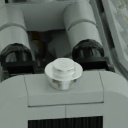
\includegraphics[width=\imagewidth]{Figures/sp_examples/sp00.jpg}%
  \label{fig:sp00}%
}\hspace{\hspacesize}%
\subfloat[snímek 1]{%
  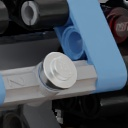
\includegraphics[width=\imagewidth]{Figures/sp_examples/sp01.jpg}%
  \label{fig:sp01}%
}\hspace{\hspacesize}%
\subfloat[snímek 2]{%
  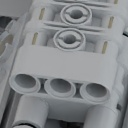
\includegraphics[width=\imagewidth]{Figures/sp_examples/sp02.jpg}%
  \label{fig:sp02}%
}

% Row 2
\subfloat[snímek 3]{%
  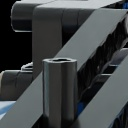
\includegraphics[width=\imagewidth]{Figures/sp_examples/sp03.jpg}%
  \label{fig:sp03}%
}\hspace{\hspacesize}%
\subfloat[snímek 4]{%
  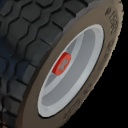
\includegraphics[width=\imagewidth]{Figures/sp_examples/sp04.jpg}%
  \label{fig:sp04}%
}\hspace{\hspacesize}%
\subfloat[snímek 5]{%
  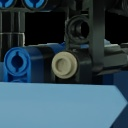
\includegraphics[width=\imagewidth]{Figures/sp_examples/sp05.jpg}%
  \label{fig:sp05}%
}

% Row 3
\subfloat[snímek 6]{%
  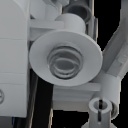
\includegraphics[width=\imagewidth]{Figures/sp_examples/sp06.jpg}%
  \label{fig:sp06}%
}\hspace{\hspacesize}%
\subfloat[snímek 7]{%
  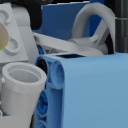
\includegraphics[width=\imagewidth]{Figures/sp_examples/sp07.jpg}%
  \label{fig:sp07}%
}\hspace{\hspacesize}%
\subfloat[snímek 8]{%
  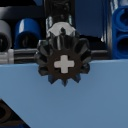
\includegraphics[width=\imagewidth]{Figures/sp_examples/sp08.jpg}%
  \label{fig:sp08}%
}

% Row 4
\subfloat[snímek 9]{%
  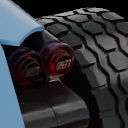
\includegraphics[width=\imagewidth]{Figures/sp_examples/sp09.jpg}%
  \label{fig:sp09}%
}\hspace{\hspacesize}%
\subfloat[snímek 10]{%
  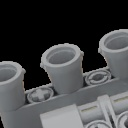
\includegraphics[width=\imagewidth]{Figures/sp_examples/sp10.jpg}%
  \label{fig:sp10}%
}\hspace{\hspacesize}%
\subfloat{%
  \hspace{\imagewidth}
}

\caption[Příklady syntetických snímků z datasetu]{Příklady syntetických snímků z datasetu, klíčový bod se nachází ve všech obrázcích uprostřed. Syntetické snímky viditelně obsahují černé pozadí, což je rozdílem oproti reálným snímkům. }
\label{fig:synthetic_images}
\end{figure}

Na obrázku \ref{fig:synthetic_images} je zřetelné, že se různé třídy klíčových bodů nacházejí i na vzájemně podobných nebo identických částech stavebnice modelu. Nejlepším příkladem může být klíčový bod 0 a klíčový bod 1. Klíčové body také i nabírají podobných tvarů, většinou kruhových. Tato povaha tříd klíčových bodů představuje jistou formu náročnosti pro modely strojového učení.

\endinput
\chapter{Návrh řešení}
\label{sec:Chapter4}
V této kapitole si přiblížíme detailnější technické údaje ohledně sítí z řad U-Net, které byly v rámci této práce implementovány. Konkrétně se jedná o U-Net, U-Net++ a pokus této práce o zařazení STN modulu do sítě U-Net.

Součástí je detailní popis augmentace trénovacích dat, rozvedení všech operací sítě, volba způsobu trénování pomocí vlastní ztrátové funkce a výsledná interpretace výstupu našich sítí. Kapitola slouží jako dostatečně přesný popis postupu následně použitých v implementační části této práce.
\endinput
\section{Augmentace dat}
\label{sec:Chapter41}
Pro účely trénování všech implementovaných neuronových sítí v této práci bylo využito augmentace trénovacích dat. Augmentace těchto snímků slouží pro představení náhodně upravených grafických odchylek během zpětné propagace sítě. Slouží pro syntetické zvětšení rozsahu datasetu a představení jistých neperfektních elementů. Tento častý přístup pak slouží k více robustní schopnosti následně vykonávat svůj úkol na reálných snímcích. Identický postup augmentace dat je použit i během následných evaluacích modelů. Mezi tyto augmentace patří:
\begin{enumerate}
  \item \textbf{Barevnost} (ang. saturation) - úprava na základě odchylky max. 10 \% oproti původní hodnotě
  \item \textbf{Světelnost} (ang. brightness) - úprava na základě odchylky max. 10 \% oproti původní hodnotě
  \item \textbf{Barevná škála} (ang. hue) - úprava RGB škály na základě odchylky max. 5 \% oproti původní hodnotě
  \item \textbf{Gaussovo rozostření} - aplikováno pomocí následujícího rozdělení
  \begin{enumerate}
      \item 10\% šance na aplikování Gaussova rozostření pomocí filtru $3\times3, \sigma=1,0$
      \item 10\% šance na aplikování Gaussova rozostření pomocí filtru $5\times5, \sigma=1,0$
  \end{enumerate}
  \item \textbf{Náhodný šum} - úprava pixelů o maximálně 3 \% (0.03) hodnoty $\sigma$ směrodatné odchylky.
\end{enumerate}
\endinput
\section{Obecný návrh sítí}
\label{sec:Chapter42}
V každém bloku se nachází dvě konvoluční operace o velikosti filtru $3\times3$, jednotným krokem v obou směrech os a ReLU aktivační funkcí. Pro všechny konvoluční operace bylo aplikováno místo odsazení typu valid padding odsazení typu same padding oproti původní architektuře \cite{unet} pro zachování velikosti obrazu na vstupu a výstupu sítě jako celku.

Pro konvoluční vrstvy s aktivační funkcí ReLU byly použity kernelové inicializéry typu \textit{He Normal}, které jsou často používány pro vrstvy s aktivační funkcí ReLU \cite{relu_henormal} a je to také i konzistentní nastavení s například oficiální implementací U-Net++ \cite{unetpp_github}. 

V blocích enkodéru se v naší implementaci používá $2\times2$ vrstva typu max pooling a $2\times2$ vrstva typu up-sampling zase v blocích dekodéru. Vrstva typu up-sampling tvoří náhradu pro původní vrstvu typu transpose. Toto rozhodnutí prane z úsudku založeném na uspokojivých výsledcích experimentálních modelů. 

\begin{figure}[ht]
    \centering
    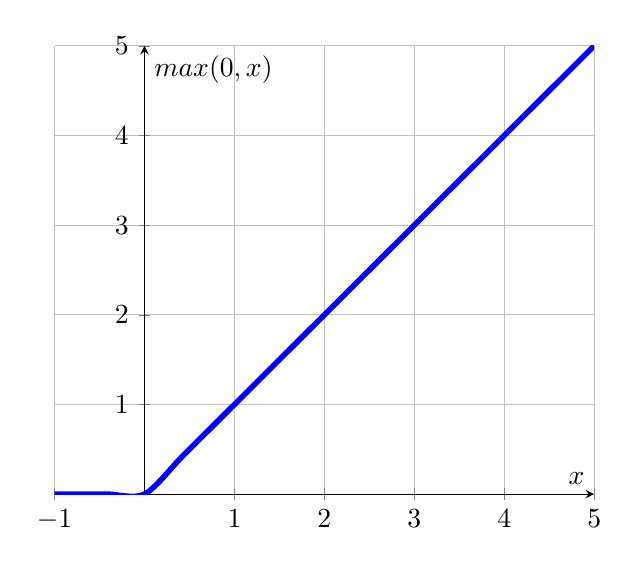
\begin{tikzpicture}
    \begin{axis}[
        axis lines=middle,
        xlabel={$x$},
        ylabel={$max(0, x)$},
        ymin=0, ymax=5,
        xmin=-1, xmax=5,
        xtick={-1,0,...,5},
        ytick={0,1,...,5},
        grid=major,
    ]
    \addplot[blue,smooth,line width=2pt] {max(0, x)};
    \end{axis}
    \end{tikzpicture}
    \caption[Aktivační funkce ReLU]{Aktivační funkce ReLU}
    \label{fig:relu}
\end{figure}

Pro každou z 2 konvolučních vrstev v rámci bloku bylo rozhodnuto aplikovat dávkovou normalizaci (ang. batch normalization), jelikož byl dokázán její pozitivní vliv ve většině případů v sítích U-Net \cite{unetnormalization}. Dávková normalizace je aplikována po konvoluční operaci a před aktivační funkcí. Dávková normalizace nebyla aplikována po finální výstupní $1\times1$ konvoluční vrstvě, a to na základě úvahy představení možného detrimentálního efektu na poslední trénovatelnou část sítě generující finální mapu příznaků, kde již nenásleduje žádná další vrstva.

Finální vrstva sítě je navržena pomocí $1\times1$ konvoluční operace na finálním bloku dekodéru. Finální vrstva má na výstupní mapě příznaků původní výšku a šířku vstupního snímku sítě, což je dosaženo pomocí aplikace odsazení typu same padding. Výstup generuje separátní mapy příznaků pro každou třídu klíčových bodů, kterých je v této práci 11. Dále v této práci jsou tyto výstupní mapy příznaků referovány jako výstupní kanály.

Pro učení se používá Gaussova funkce s pevně nastavenou hodnotou $\sigma$ a je to i výstupem trénovatelné části sítě. Detailní informace týkající se výstupu sítě a sítí následujících v této práci je detailněji popsáno v kapitole \ref{sec:Chapter46}.
\endinput
\section{Řešení pomocí sítě U-Net}
\label{sec:Chapter43}
Jako náš první základní model volíme síť standardní U-Net architektury navazující na původní architekturu představenou v \cite{unet}. Byl zvolen přístup 4 bloků jak enkodéru, tak symetricky i dekodéru. Architektura může být znázorněna pomocí následující tabulky \ref{fig:model_architecture}:

\begin{table}[ht]
\centering
\begin{tabular}{@{}lrr@{}}
\toprule
Typ vrstvy & Počet filtrů & Velikost filtru \\ \midrule
$2\times$ Conv2D+BN+ReLU & 32 & $3 \times 3$ \\
MaxPooling2D & - & $2 \times 2$ \\
$2\times$ Conv2D+BN+ReLU & 64 & $3 \times 3$ \\
MaxPooling2D & - & $2 \times 2$ \\
$2\times$ Conv2D+BN+ReLU & 128 & $3 \times 3$ \\
MaxPooling2D & - & $2 \times 2$ \\
$2\times$ Conv2D+BN+ReLU & 256 & $3 \times 3$ \\
MaxPooling2D & - & $2 \times 2$ \\
$2\times$ Conv2D+BN+ReLU & 512 & $3 \times 3$ \\
UpSampling2D & - & $2 \times 2$ \\
$2\times$ Conv2D+BN+ReLU & 256 & $3 \times 3$ \\
UpSampling2D & - & $2 \times 2$ \\
$2\times$ Conv2D+BN+ReLU & 128 & $3 \times 3$ \\
UpSampling2D & - & $2 \times 2$ \\
$2\times$ Conv2D+BN+ReLU & 64 & $3 \times 3$ \\
UpSampling2D & - & $2 \times 2$ \\
$2\times$ Conv2D+BN+ReLU & 32 & $3 \times 3$ \\
% Final output layer
Conv2D+Sigmoid & 11 & $1 \times 1$ \\
\bottomrule
\end{tabular}
\caption[Konvoluční a pooling vrstvy implementace sítě U-Net]{Konvoluční a pooling vrstvy implementace sítě U-Net, kde Conv2D je konvoluční operace a BN je zkratkou pro dávkovou normalizaci (ang. batch normalization). }
\label{fig:model_architecture}
\end{table}

Ve finále tato síť bez parametrů optimizéru či uložených gradientů dosahuje velikosti 7 852 875 parametrů (okolo 30 MB).


\endinput
\section{Řešení pomocí sítě U-Net++}
\label{sec:Chapter44}
Síť U-Net++ se odvíjí od architektury U-Net v předchozí kapitole \ref{sec:Chapter43}, rozšiřující její možnosti a sémanticky propojující části enkodéru a dekodéru svými skokovými bloky \cite{unetpp}. Jako v předchozí kapitole, rozhodujeme se pro volbu 4 bloků enkodéru a dekodéru, počínající od počtu 32 filtrů po 256 filtrů v poslední bloku enkodéru a prvním bloku dekodéru, s krkem obsahující 512 filtrů. Obecné návrhy popsány v kapitole \ref{sec:Chapter42} jsou obdobně použity i pro hluboké skokové bloky přidány v rámci sítě U-Net++ \cite{unetpp}.

Skokové bloky přidány v této síti jsou přidány mezi vrstvy dekodéru a enkodéru v rámci pokusu vylepšení výsledků původní sítě U-Net. Premise a detaily vylepšení této sítě jsou detailně popsány v kapitole \ref{sec:Chapter23}. Přesné vyobrazení implementované sítě je graficky reprezentováno v části (b) obrázku \ref{fig:unetpp}. Inspirace pro implementační detaily této sítě plynou také z open-source implementace citované v originální literatuře \cite{unetpp_github}.

Síť je trénována v režimu hluboké supervize na základě výstupu bloků $X^{0,1}$, $X^{0,2}$, $X^{0,3}$, $X^{0,4}$ (jejich ztrátové hodnoty jsou sečteny a tato hodnota je minimalizována optimizérem). Samozřejmě ztrátová funkce nepracuje s ReLU výstupy, ale pro každý blok účastnící se hluboké supervize byla přidána $1\times1$ finální konvoluční vrstva. Při trénování modelu bez hluboké supervize pomocí standardního přístupu zpětné propagace na finální vrstvě se ztrátové funkce účastní pouze finální blok dekodéru $X^{0, 4}$.

Pro U-Net++ se v režimu hluboké supervize očekává průměrování na výsledných výstupech zúčastěných bloků. Tato možnost bude vyzkoušena v implementační a evaluační části práce a porovnána s výsledky výstupu jednotného bloku $X^{0, 4}$ také v rámci hluboké supervize.

Síť U-Net++ obsahuje ve verzi s hlubokou supervizí 9 164 748 parametrů a 9 163 659 v režimu bez hluboké supervize, což je zhruba 17\% nárůst velikosti sítě oproti síti U-Net. Velikost v obou případech dosahuje velikosti zhruba 35 MB.
\endinput
\section{Řešení pomocí sítě U-Net STN}
\label{sec:Chapter45}
U-Net STN není přesným názvem pro ustálenou architekturu neuronové sítě, avšak název zvolen v rámci této práce pro experiment o zařazení modulu STN (popsaného v kapitole \ref{sec:Chapter28}) do sítě U-Net (popsanou v kapitole \ref{sec:Chapter22}). Pomocí přirozeného úsudku jsem zvolil modul STN vložit jako první část sítě, předcházející enkodér a následné vrstvy. Premisí zařazení tohoto modulu, které by mohly vylepšit výsledky původní architektury U-Net, může být hned několik:
\begin{enumerate}
    \item \textbf{Lepší prostorová invariance} -- Jelikož klasické přístupy pomocí konvolučních neuronových sítí (CNN) relativně postrádají invarianci vůči prostorovým změnám \cite{stn}, modul STN se může naučit převést vstupní snímek do více generalizované formy, jinak řečeno lépe \enquote{chápatelné} a zpracovatelné pro následující vrstvy sítě navazující na výstup modulu STN. Toto také může teoreticky vést i ke zlehčení lokalizační a klasifikační úlohy pro následnou síť U-Net díky přenosu této zodpovědnosti ze sítě U-Net do modulu STN. Tímto se tyto 2 obecné části mohou k sobě stát komplementárními, což zlepšuje obecnou robustnost této sítě jako celku.
    \item \textbf{Představení mechanizmu pozornosti} -- Modul STN se může naučit během tréninku lépe identifikovat důležité části snímku a předpovědět, v jaké oblasti na snímku bude pravděpodobně probíhat lokalizační úloha. Díky tomu se může modul několika způsoby pokusit o představení pozornosti na tuto oblast, a to jak například pomocí přiblížení na tuto oblast (pomocí škálovacích parametrů transformační matice $\theta$), tak i pomocí přesunutí této oblasti do středu výstupní mapy.
    \item \textbf{Ko-lokalizátor} -- Funkce modulu STN jako ko-lokalizátor souvisí s mechanizmem pozornosti a jedná se tedy pouze o přímou implikaci této schopnosti na možnost již už také hrubě rozeznat klíčové body. I když trénovatelná část modulu STN není nijak propojená s následnou sítí U-Net a nemohou sdílet informace v tradičním smyslu propojených vrstev neuronových sítí, modul STN může již jednoduché lokalizační úlohy hrubě lokalizovat a následně je například převést do středu snímku.
\end{enumerate}

Pro pokus o zařazení modulu STN může být zvolen přístup kompletní afinní 2D transformace pomocí 6 parametrů $\theta$ (matice \ref{eq:stn_6_theta}), nebo pomocí pouze 3 parametrů $\theta$ (matice \ref{eq:stn_3_theta}). Obraz je pomocí vzorkovníku na daných parametrech transformován a předán dále do sítě U-Net, tedy do prvního bloku enkodéru. Síť U-Net je v tomto přístupu stavěna identicky jako v předchozím přístupu v kapitole \ref{sec:Chapter43}.

\subsection{Návrh lokalizační sítě STN}

\textbf{Lokalizační síť} modulu STN je v případě této práce navržena jako síť typu CNN s navazující regresní sítí plně propojených vrstev (ang. dense layer). V následující tabulce \ref{fig:stn_loc_net} je popsána zvolená architektura. $m$ je referenční hodnota pro počet jednotek a filtrů, stanovena na hodnotu $128$ a $n_{\theta}$ zase určuje počet výstupních parametrů $\theta$, v rámci praktické části této práce $3$ a $6$:

\begin{table}[H]
\centering
\begin{tabular}{@{}llrr@{}}
\toprule
Typ vrstvy & Aktivační funkce & Počet filtrů / jednotek neuronů & Velikost filtru \\ \midrule
Conv2D & ReLU & $m$ & $3 \times 3$ \\
MaxPooling2D & - & - & $2 \times 2$ \\
Conv2D & ReLU & $2\times m$ & $3 \times 3$ \\
MaxPooling2D & - & - & $2 \times 2$ \\
Conv2D & ReLU & $4\times m$ & $3 \times 3$ \\
MaxPooling2D & - & - & $2 \times 2$ \\
GlobalAverageMaxPooling & - & - & - \\
\bottomrule
Dense & ReLU & $4\times m$ & - \\
Dense & ReLU & $2\times m$ & - \\
Dense & ReLU & $n_{\theta}$ & - \\
\bottomrule
\end{tabular}
\caption[Návrh lokalizační sítě modulu STN] { Návrh lokalizační sítě modulu STN }
\label{fig:stn_loc_net}
\end{table}

\subsection{Návrh vzorkového pole}

V modulu STN je v druhé částí generátor vzorkového pole. Generátor vzorkového pole má zodpovědnost generovat vzorkovou mapu $T_{\theta}(G)$ z jednotkové vzorkové mapy $T_{I}(G) = G$ (viz obrázek \ref{fig:stn_grid}), která je v normalizovaném rozsahu $\langle-1, 1\rangle$ pro určení středu souřadného systému doprostřed snímku. Vzorková mapa $T_{\theta}(G)$ se generuje pomocí matice $\displaystyle \mathrm {A}_\theta$. 

Výsledné vzorkové pole $T_{\theta}(G)$ následně vstupuje do vzorkovníku, který na vstupní snímek aplikuje pomocí bilineární interpolace finální transformaci generující výstupní snímek modulu STN.

\subsection{Způsob tréninku}

Síť U-Net STN může být natrénovaná několika způsoby. V datasetu jsou dostupné syntetické snímky s již transformovaným klíčovým bodem do normalizované podoby, včetně komplementární informace o rotaci a škálování použité k transformaci pravých snímků do syntetických. Modul STN můžeme trénovat separátně, nebo také i v tzv. režimu end-to-end v rámci celé sítě U-Net STN.

Pro U-Net STN byl zvolen přístup v režimu \textbf{tzv. end-to-end a bez přímé supervize} čili jsme se rozhodli nepoužít dodatečné informace datasetu a parametry $\theta$ přímě neaplikovat ve výpočtu ztrátové funkce. Modul STN se ve fázi tréninku sítě tedy pokusí o nalezení nejlepšího způsobu transformací pro finální lokalizační úlohu.

\endinput
\section{Výstup sítí}
\label{sec:Chapter46}
\subsection{Výstupní vrstva}
Jak bylo již řečeno v předchozích sekcích o návrhů sítí U-Net, U-Net++ a U-Net STN, finální vrstvou je vždy konvoluční operace $1\times1$ s aktivační funkcí sigmoid generující mapu příznaků ekvivalentní velikosti jako je vstupní obraz. V této práci používáme 11 tříd pro lokalizaci, kde lokalizace probíhá na každém jednotlivém filtru pro daný kanál separátně, čili velikost výstupu je velikost vstupního obrázku (díky odsazení typu same padding) o hloubce 11 kanálů.

Aktivační funkce sigmoid je funkce, která se používá v neuronových sítích k převodu vstupních hodnot na hodnoty v rozmezí 0 a 1. Je definována vzorcem:

\begin{equation}
\sigma(x) = \frac{1}{1+e^{-x}}\,,
\end{equation}
kde $e$ je základ přirozeného logaritmu (Eulerovo číslo) a $x$ je vstupní hodnota. Tato funkce je obzvláště užitečná pro úlohy s binární povahou. Každý kanál tedy můžeme chápat jako binární softmax klasifikátor na úrovni pixelů, kde relativní vzdálenost od výskytu daného klíčového bodu je hodnota daného pixelu.

\begin{figure}[H]
    \centering
    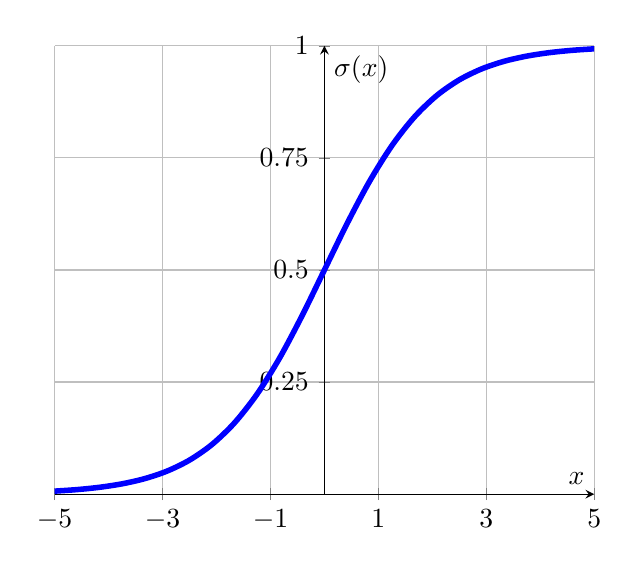
\begin{tikzpicture}
    \begin{axis}[
        axis lines=middle,
        xlabel={$x$},
        ylabel={$\sigma(x)$},
        ymin=0, ymax=1,
        xmin=-5, xmax=5,
        xtick={-5,-3,...,5},
        ytick={0,0.25,...,1},
        grid=major,
    ]
    \addplot[blue,smooth,line width=2pt] {1/(1+exp(-x))};
    \end{axis}
    \end{tikzpicture}
    \caption[Aktivační funkce sigmoid]{Aktivační funkce sigmoid}
    \label{fig:sigmoid}
\end{figure}

Toto vede k možnosti jednoduše provést lokální klasifikaci na jednotlivých kanálech, a to s pomocí maximální nalezené hodnoty na výstupním kanálu (což je typicky z praktického hlediska i hledaná pozice klíčového bodu). Například výstupní kanál s maximální hodnotou 0,8 vykazuje silnou pravděpodobnost výskytu klíčového bodu na daném kanálu oproti kanálu s max. hodnotou 0,3.

\subsection{Reprezentace klíčových bodů}

Jako reprezentaci klíčových bodů na výstupu sítě si v tomto nastavení volíme reprezentaci Gaussovy funkce ve 2D prostoru. Gaussova funkce působí jako přirozený kandidát pro aktivační funkci sigmoid. Tato reprezentace má svou maximální hodnotu o hodnotě 1 ve svém středu, kde se nachází náš klíčový bod v době tréninku. Gaussovou funkci pro výpočet hodnot na 2D skalární mapě jako tzv. ground truth pro trénink výstupních kanálů můžeme zapsat takto:

\begin{equation}
    G(x, y) = a \exp\left(-\frac{(x - c_x)^2 + (y - c_y)^2}{2\sigma^2}\right)\,,
\end{equation}
kde $a$ je amplitudový faktor Gaussovy funkce, $x$ a $y$ jsou pozice na 2D skalárním poli, $c_x$ a $c_y$ označují souřadnice středu klíčového bodu a $\sigma$ udává směrodatnou odchylku, která ovlivňuje rozptyl Gaussovy funkce. Parametry Gaussovy funkce si volíme jako následující hodnoty pro adekvátní rozptyl na výstupních kanálech: 
\begin{itemize}
    \item pro $128 \times 128$ snímky -- $a=1$, $\sigma=$ 5,0
    % \item pro $256 \times 256$ snímky -- $a=1$, $\sigma=$ 10,0
\end{itemize}

\begin{figure}[H]
\centering
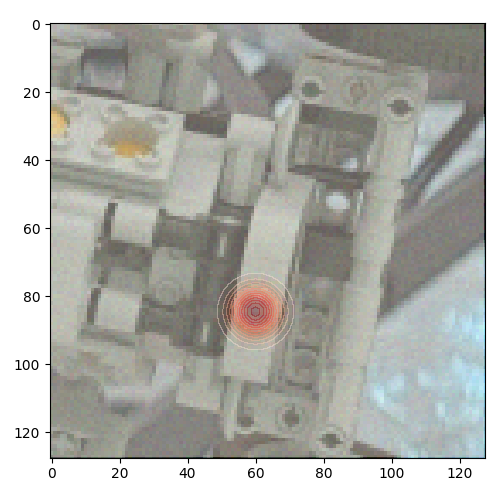
\includegraphics[width=0.3\textwidth,keepaspectratio]{Figures/kp_examples/kp_example_00.png}
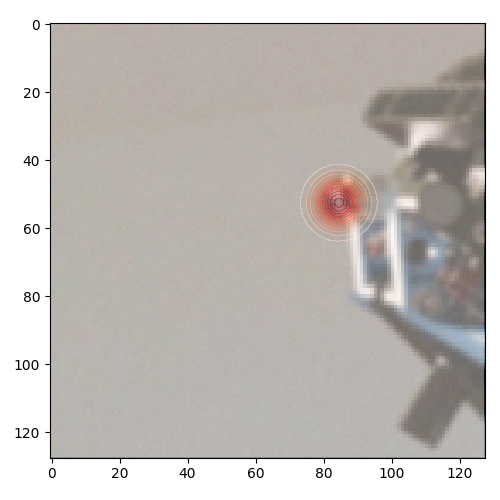
\includegraphics[width=0.3\textwidth,keepaspectratio]{Figures/kp_examples/kp_example_01.png}
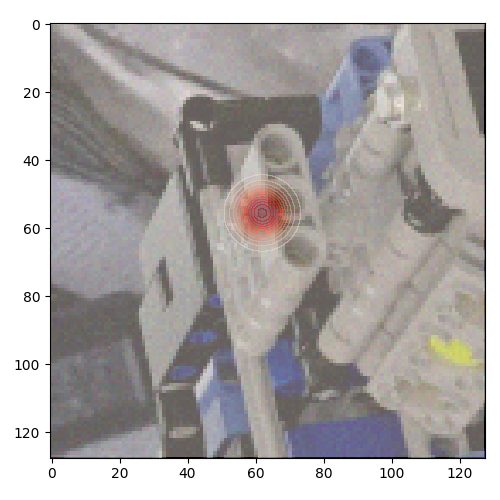
\includegraphics[width=0.3\textwidth,keepaspectratio]{Figures/kp_examples/kp_example_02.png}
\caption[Příklad aplikace Gaussovy funkce na snímky s klíčovým bodem]{Příklad aplikace Gaussovy funkce na augmentované snímky s klíčovým bodem.}
\label{fig:kp_examples}
\end{figure}

% Během experimentálních trénincích nevyskytujících se ve finálních evaluacích jsme pracovali i s premisí odebrání ReLU aktivační funkce na posledním bloku dekodéru těsně před aplikací sigmoid aktivační funkce. Tato premise se neobhájila a vyšlo najevo, že představení linearity v předposlední konvoluční operaci má detrimentální účinky na lokalizační přesnost sítě. MOŽNÁ DÁT DO DALŠÍ KAPITOLY.
\endinput
\section{Ztrátová funkce}
\label{sec:Chapter47}
Pro zpětnou propagaci všech našich modelů využíváme jako základní ztrátovou funkci střední kvadratickou chybu (MSE, Mean Squared Error), protože tato metoda penalizuje velké odchylky mezi predikovanými a skutečnými hodnotami.  V naších sítích aplikujeme globální průměrování (ang. reduce mean) s výpočtem MSE:
\begin{equation}
    loss(y_i, \hat{y}_i) = \frac{1}{N} \sum_{i=1}^{N} (y_i - \hat{y}_i)^2 \,,
\end{equation}
kde $y_i$ je konkrétní hodnota z přímého průchodu sítě na pozici $i$, $\hat{y}_i$ je kontrolní hodnota na pozici $i$ (aneb tzv. ground truth) a $N$ je celkový počet hodnot na mapě příznaků. Kontroluje se vždy pouze daný výstupní kanál ze všech 11, to kvůli povaze informacím k datasetu popsaným v kapitole \ref{sec:Chapter31}. Ve fázi tréninku také můžeme síť trénovat na již zmíněných falešných snímcích, neobsahující klíčový bod dané třídy na odpovídajícím výstupní kanálu - zde můžeme trénovat opět pouze na daném kanálu, opět ze stejného důvodu jako při pravých snímcích.

\subsection{První návrh ztrátové funkce}

První návrh pro trénování sítě byl rozdělit poměr výskytu pravých a falešných snímků při tréninku na $50:50$. I když se může řešení ztrátové funkce zdát kompletní, zdaleka není. Při experimentech se ukázalo, a teoretická představa tomu odpovídá, že toto tréninkové nastavení zcela nezabraňuje falešným detekcím i na neodpovídajících kanálech podobných klíčových bodů. Přestože přesné lokalizace bylo dosaženo, kanály ostatních tříd klíčových bodů dosahovaly při lokalizaci na svém maximu hodnoty blížící se $1,0$.

\subsection{Pokus o adresování korektní klasifikace}

Druhý návrh pro adresování korektní klasifikace mezi kanály bylo vytvořit set klíčových bodů, mezi kterými docházelo k detekci na neodpovídajících výstupních kanálech. Konkrétně se jednalo o třídy $\{0, 1, 5, 6, 9\}$ (viz. obrázek \ref{fig:synthetic_images}). Pravé snímky těchto bodů byly aplikovány jako falešné pro ostatní snímky z tohoto setu v poměru 25 \% k celému tréninku. Na snímcích se na základě manuální vizuální kontroly nevyskytovaly pozitivní detekce navzájem mezi sebou, čili to působilo jako řešení, které by mohlo vést ke zlepšení.

I když tento přístup představil síti schopnost korektní klasifikace na daný set tříd, mezi kterými probíhala vzájemná detekce a neschopnost vzájemného odlišení, došlo k zajímavé anomálii -- síť sice nabrala schopnost odlišit daný set klíčových bodů, avšak ztratila schopnost odlišení mezi vůbec si nepodobnými klíčovými body.

\subsection{Finální podoba ztrátové funkce}
\label{subsec:Chapter473_final_loss}

Finálně bylo vyvinuto řešení, které je univerzální a je použito ve všech modelech finálně implementovaných v této práci. V průběhu tréninku sítě byl proud trénovacích dat v následujícím poměru:
\begin{enumerate}[label=(\Alph*)]
    \item 50 \% \textbf{pravé snímky} -- aplikovány na daný výstupní kanál s použitím MSE.
    \item 25 \% \textbf{falešné snímky} -- aplikovány na daný výstupní kanál s použitím MSE mezi predikovaným výstupním kanálem a nulovou 2D skalární mapou.
    \item 25 \% \textbf{snímky pro eliminaci detekcí} na ostatních 10 výstupních kanálech. Pravý snímek z datasetu se ve fázi tréninku modelu aplikuje na jakoukoli náhodnou třídu z ostatních 10 klíčových bodů. Ztrátová funkce je s pomocí masky aplikována podobně jako při falešných snímcích mezi výstupním kanálem a nulovou 2D skalární mapou, avšak pouze v daném rozsahu od klíčového bodu. Detekce na okolních oblastech ve snímku jsou tedy v tomto případě ignorovány.
\end{enumerate}
Po přidání případu (C) by se měla síť naučit korektně eliminovat detekce na nerelevantních výstupních kanálech. S případem (C) ale také v zájmu zachování udržení číselné stability, což je klíčové pro zajištění konzistentní a efektivní konvergence v procesu trénování, musíme aplikovat následující normalizaci:
\begin{equation}
loss(y_i, \hat{y}_i) = \frac{\sum_{i=1}^{N} [(y_i - \hat{y}_i)^2\times m_i]}{\sum_{i=1}^{N} m_i}\,,
\end{equation}
kde $m_i$ tvoří konkrétní binární hodnotu masky na indexu $i$, a tedy $\sum_{i=1}^{N} m_i$ počet pozitivních hodnot v masce, neboli počet bodů aplikovaných ve výpočtu ztrátové funkce. V případech (A) a (B) je to prakticky velikost výstupní mapy příznaků sítě, tj. výška$\times$šířka. V případě (C) se jedná o počet pozitivních hodnot masky.

\subsection{Přizpůsobení ztrátové funkce pro U-Net STN}
\label{subsec:Chapter474_stn_loss}

Modul STN v rámci sítě U-Net udává potřebu uzpůsobit výpočet ztrátové funkce pro transformovaný snímek, který není jednotný se vstupním snímkem. Aby se trénink mohl adaptovat na chování modulu STN s použitím předchozí ztrátové funkce, je nutno aplikovat pár změn:
\begin{itemize}
    \item \textbf{Transformace klíčového bodu} - generace kontrolní mapy příznaků se v případě U-Net STN stává úloha, která nemůže být provedena před průchodem sítí na daném snímku. Gaussova funkce musí být vygenerována na pozici transformovaného klíčového bodu pomocí známých parametrů $\theta$ ve fázi výpočtu ztrátové funkce během tréninku. Pokud bychom s předchozím nastavením ztrátové funkce spustili trénink sítě U-Net v režimu s použitím modulu STN, dosáhli bychom prakticky identických výsledků jako v klasické sítí U-Net, pouze s delší dobou konvergence. STN modulu by bylo znemožněno provádět drtivou většinu transformací.
    \item \textbf{Omezení souřadnic klíčového bodu} - zajímavým důsledkem při tzv. end-to-end tréninku sítě s modulem STN bez přímé supervize je možnost přeučení díky schopnosti dynamicky upravit vstupní data. Modul STN se bez aplikace omezení souřadnic klíčového bodu velmi rychle naučí hledaný klíčový bod transformovat mimo rozsah vstupního snímku. Při použití s originální ztrátovou funkcí v kapitole \ref{subsec:Chapter473_final_loss} se poté transformují i hodnoty masky $m$ a výpočet ztrátové funkce se tímto díky přeučení zablokuje, dosahujících hodnot silně se blížících 0, a vznikne kompletní odmítnutí sítě provádět lokalizační úlohu. Souřadnice byly omezeny na rozsah normalizovaného souřadnicového systému [0,9; 0,9] původního rozsahu [1,0; 1,0]. Od těchto hranic snímku se přidává lineární penalizační ztrátová hodnota na základě součtu přesahu transformovaného správného klíčového bodu na snímku na obou dvou osách:
    \begin{equation}
    \begin{aligned}
    P(a_x, a_y) = & \max(0, a_x - \alpha) + \max(0, -\alpha - a_x) \\
                  & + \max(0, a_y - \alpha) + \max(0, -\alpha - a_y)\,,
    \end{aligned}
    \end{equation}
    kde $(a_x, a_y)$ je transformovaná hodnota správného klíčového bodu dle matice ${\displaystyle \mathrm {A} }_\theta$ a $\alpha =$ 0,9 specifikuje hranice rozsahu transformovaného správného klíčového bodu.
    
\end{itemize}

Výsledná ztrátová funkce pro U-Net STN by tedy mohla vypadat následovně:
\begin{equation}
\begin{aligned}
loss(y_i, \hat{y}_i) = & \frac{\sum_{i=1}^{N} [(y_i - \hat{y}_i)^2\times m_i]}{\sum_{i=1}^{N} m_i} + P(a_x, a_y).
\end{aligned}
\end{equation}

\endinput
\chapter{Implementace a experimenty}
\label{sec:Chapter5}
V této kapitole nalezneme již konkrétní vysvětlení od popisu systému uzpůsobeného pro tuto práci až po popis finální implementace těch nejdůležitějších aspektů návrhů a tréninků našich sítí, včetně mapovacích funkcí, ztrátových funkcí a STN modulu. 

Součástí této kapitoly je detailní přiblížení včetně útržků zdrojových kódů. Implementace následujících zdrojových kódů uvedené v následující kapitole vycházejí na základě implementace pomocí oficiální dokumentace TensorFlow a Keras \cite{tensorflow_doc}. Všechny tyto zdrojové kódy je možno najít v kompletním znění v příloze. Jediným rozdílem je experiment s použitím DINOv2, který funguje na knihovně PyTorch.

\endinput
\section{Jazyky a prostředí}
\label{sec:Chapter51}
V rámci této práce jsem se pohyboval primárně v prostředí jazyka \textbf{Python}, což je skvělá volba pro rychlé, spolehlivé, nastavitelné a silně modulární nastavení v oblasti strojového učení. S jazykem Python jsme používali nástroje virtuálních prostředí \textit{pip} a \textit{Anaconda}, které spravovaly balíčky jazyka Python pro tuto práci

Pro vývoj byla použita verze Python 3.10 na operačním systému Ubuntu 22.04.03 LTS\footnote{Dlouhodová podpora, ang. Long Time Support.}. Operační systém Ubuntu nebyl první volbou. První volbou bylo prostředí Debian 12. Avšak ukázalo se, že budování prostředí co se týče balíčkovacích kompatibilit mezi verzemi ovladačů, verzemi balíčků pro Python a verzemi cuDNN\footnote{Knihovna zprostředkující jazyk CUDA grafických karet NVIDIA pro účely strojového učení.} bylo co se týče instalace a nastavení nejvíce vyhovující na prostředí Ubuntu, což bylo doporučeno i dokumentací následně zmíněných knihoven (jako je např. TensorFlow).

Toto prostředí nebylo virtualizováno, nebylo využito prostředků jako je např. Docker a tento systém byl uzpůsoben přímo pro využití v analýze dat a strojového učení.

Většina experimentálního trénování proběhla na následujícím hardwaru:

\begin{table}[hb]
\centering
\begin{tabular}{@{}lll@{}}
\toprule
Součást & Model \\
\midrule
CPU & AMD Ryzen 5 7600 6-core processor \\
GPU & NVIDIA GTX 1070 Strix 8GB VRAM  \\
RAM & 32 GB 6000MHz DDR5 \\
\bottomrule
\end{tabular}
\caption{Domácí systém pro trénink}
\label{fig:wortelus_pc}
\end{table}
\endinput
\section{Trénovací API}
\label{sec:Chapter52}
Pro trénink, export, inferenci a všechny ostatní manipulace s modely byla použita knihovna TensorFlow 2.13.0. Na základě této knihovny jsem vyvinul svou kódovou bázi pro účely strojového učení této práce fungující primárně na příkazové řádce pro trénink, evaluaci, generaci metrik a grafů, ale i interaktivní inferenci. Tato kódová báze sloužila jako pracovní nástroj pro práci se sítěmi aplikovanými v této práci. Společně s knihovnou TensorFlow byly využity přídavné moduly jako je např. \textit{tensorflow-addons}, \textit{tensorflow-probability} \cite{tensorflow_libs} pro využití při programování částí tréninku či inference či \textit{TensorRT} \cite{tensorrt_docs} sloužící pro zlepšení inferenčního výkonu a rychlosti.
\endinput
\section{Dodatečné nástroje}
\label{sec:Chapter53}
Pro práci s modely, výsledky modelů, datasetem, zpracováváním dat obecně atd. bylo použito několika nástrojů komplementárním k postupu na úlohách řešených v rámci této práce, mezi ně patří:

\endinput
\section{Průběh tréninku}
\label{sec:Chapter54}
Tréninky byly spouštěny ve stavech specifikovaných v kapitole \ref{sec:Chapter53} na stroji popsaném v kapitole \ref{sec:Chapter51}. Pro trénink byly v prostředí \texttt{Keras} použity zpětné volání a výstupy pro:
\begin{itemize}
    \item Včasné zastavení pro případ nezlepšení výsledků validační ztráty mezi epochami, nastaveno na 3 epochy.
    \item Ukládání snímku trénovatelných vah a gradientů z dosavadně nejlepší epochy dle validační ztráty - \texttt{best.ckpt}
    \item Ukládání snímku trénovatelných vah a gradientů z poslední epochy dle validační ztráty - \texttt{cp.ckpt}
    \item Zaznamenování trénovacích a validačních ztrátových hodnot
    \item Trénovací a validační výstup pro nástroj \texttt{TensorBoard}
\end{itemize}
Během tréninku jsme díky použití několika verzí architektur sítí s úpravami ve ztrátových funkcích zastavovali model i manuálně při signifikantním nezlepšení ztrátové hodnoty. Ve všech případech byl pro výsledný model zvolen tzv. checkpoiint s nejlepší validační ztrátou.
\endinput
\section{Detaily implementace}
\label{sec:Chapter55}

\subsection{Preprocessing dat}
Funkce \texttt{tf.Dataset.map(lambda line: decode\_csv\_line(line))} tvoří první krok proudu dat při tréninku všech našich sítí. Mapovací funkce datasetu se stará o tyto kroky, v následujícím pořadí:
\begin{enumerate}
    \item \textbf{Náhodný výběr trénovacího způsobu} - pomocí pravidla $50:25:25$ je vybrán jeden ze 3 trénovacích způsobů popsaných blíž v kapitole \ref{subsec:Chapter473_final_loss}.
    \item \textbf{Preprocessing a augmentace snímků} - snímky jsou načteny a augmentovány o náhodné změny popsané blíž v kapitole \ref{sec:Chapter3}.
    \item \textbf{Generace mapy příznaků} - generace mapy příznaků pro relevantní zvolenou trénovací úlohu. V rámci tréninku sítě U-Net STN se tento krok provádí ve ztrátové funkci.
    \item \textbf{Generace masky} - generace relevantní masky pro danou trénovací úlohu. V rámci tréninku sítě U-Net STN se tento krok provádí ve ztrátové funkci.
    \item \textbf{Tvorba výstupu} - augmentovaný vstupní snímek, tak koplementární data do ztrátové funkce jsou výstupem mapovací funkce.
\end{enumerate}

Mapovací funkce datasetu použitých v této práci jsou k nalezení v příloze v souborech \texttt{map.py} a \texttt{map\_stn.py}.



\subsection{Ztrátová funkce}
\label{subsec:Chapter55_loss_func}

Pro trénink modelů U-Net a U-Net++ byla ztrátová funkce dle kapitoly \ref{subsec:Chapter473_final_loss} vytvořena do následující podoby \ref{src:loss_func}. Ztrátová funkce je samozřejmě konstruována vektorizovaným způsobem:

\label{src:loss_func}
\lstinputlisting[language=Python, caption={Ztrátová funkce pro pro sítě U-Net a U-Net++}]{SourceCodes/loss.py}

\subsection{Ztrátová funkce pro U-Net STN}
\label{subsec:Chapter55_loss_func_stn}

Pro použití modulu STN musely být aplikovány úpravy, detailněji popsány v kapitole \ref{subsec:Chapter474_stn_loss}. Zmíněná transformace správného klíčového bodu dle parametrů $\theta$ je ve ztrátové funkci uzpůsobena následovně s použitím pomocného výstupu z modulu STN \texttt{theta}. Ve fázi tohoto výpočtu je souřadnicový systém v normalizované formě.

\label{src:loss_func_stn_inv_pos}
\lstinputlisting[language=Python, caption={Útržek z end-to-end ztrátové funkce sítě U-Net STN pro transformaci lokace správného klíčového bodu do nové lokace na základě affiní transformační matice theta. }]{SourceCodes/loss_stn_inv_pos.py}

Výsledné souřadnice jsou pak následně převedeny zpět do původního souřadnicového systému rozsahu snímku v pixelech. Na základě těchto souřadnic jsou vygenerovány mapy příznaků a masky sloužící pro výpočty ve ztrátové funkci, která je obdobná s klasickou implementací v předchozí kapitole \ref{subsec:Chapter55_loss_func}.

Normalizované transformované souřadnice jsou také využity pro výpočet pomocné ztráty:
\label{src:loss_stn_aux_func}
\lstinputlisting[language=Python, caption={Pomocná ztrátová funkce pro supervizi lokace normalizovaných transformovaných souřadnic na snímku. }]{SourceCodes/loss_stn_aux.py}

\endinput
\section{Modul STN}
\label{sec:Chapter56}
Modul STN je tvořen jako vlastní Keras vrstva dědící z \texttt{tf.keras.layers.Layer}. Metoda \texttt{call(inputs)}\footnote{Metoda vrstvy pro transformaci vstupu přímým průchodem sítí.} je navržena takto:

\label{src:stn_call}
\lstinputlisting[language=Python, caption={Metoda \texttt{call(inputs)} }]{SourceCodes/stn.py}

Funkce \texttt{bilinear\_sampler(inputs, xS, yS)} pro tvorbu vzorkovacího pole je tvořena následovně:

\label{src:stn_grid_gen}
\lstinputlisting[language=Python, caption={Metoda \texttt{bilinear\_sampler(inputs, xS, yS)} }]{SourceCodes/stn_grid_gen.py}

\endinput
\chapter{Výsledky a zhodnocení}
\label{sec:Chapter6}
V rámci této práce bylo implementováno 5 modelů konvolučních neuronových sítí:
\begin{enumerate}
    \item \textbf{U-Net}
    \item \textbf{U-Net++ bez hluboké supervize} 
    \item \textbf{U-Net++ s hlubokou supervizí}
    \item \textbf{U-Net STN 3-parametrový} - verze modelu U-Net s modulem STN a 3 výstupními parametry $\theta$.
    \item \textbf{U-Net STN 6-parametrový} - verze modelu U-Net s modulem STN a 6 výstupními parametry $\theta$.
\end{enumerate}
V této kapitole si přiblížíme zjištění, výsledky, metriky a evaluace těchto modelů.

\endinput
\section{Časy tréninku a inference}
\label{sec:Chapter61}
V následující tabulce \ref{tab:models_performance} můžeme vidět výkon trénovaných modelů na našem hardwaru (popsaném v \ref{fig:wortelus_pc}):
\begin{table}[H]
    \centering
    \begin{tabular}{lrrrr}
        \toprule
         & Čas trénovací ep. & Celkem ep. & Nejlepší ep. & Inference \\
         \midrule
         U-Net & 29:04 & 16 & 15 & 8 ms \\
         U-Net++ bez HS & 1:12:25 & 25 & 25 & 9 ms \\
         U-Net++ s HS & 1:15:03 & 22 & 22 & 10 ms \\
         U-Net STN 3-parametrový & 42:52 & 19 & 16 & 13 ms \\
         U-Net STN 6-parametrový & 42:59 & 22 & 19 & 13 ms \\
         \bottomrule
    \end{tabular}
    \caption[Statistiky trénovaných modelů]{Časy trénovacích epoch (bez validace) na NVIDIA GTX 1070 Strix 8 GB společně s inferenčním časem a výběrem epoch. }
    \label{tab:models_performance}
\end{table}

\endinput

\chapter{Závěr}
\label{sec:Chapter7}
Hlavním cílem této práce byla rešerše přístupů k lokalizaci klíčových bodů pomocí hlubokých neuronových sítí a následný pokus implementace vybraných modelů. Modely byly úspěšně implementovány pomocí knihovny a učícího API TensorFlow v jazyce Python 3.

Práce byla zaměřena primárně na architektury hlubokých konvolučních neuronových sítí U-Net. Implementována byla síť U-Net a U-Net++. Byl i vytvořen v rámci této práce model U-Net STN a vyzkoušení jeho výkonu na testovacích syntetických a reálných snímcích.

Model U-Net dosáhl obstojných výsledků a představení modulu STN do sítě U-Net ukázalo zajímavé zlepšení zejména v přesnosti lokalizace na testovacím datasetu. Nejlépe si obstojila síť s hlubší architekturou \textbf{U-Net++ bez použití hluboké supervize}, která dosáhla nejnižšího počtu falešných detekcí a průměru chyby lokalizace (0,69 $\pm$ 1.20). Dosáhla také lepších výsledků při zkouškách na reálně vyfocených snímcích. \textbf{Síť DINOv2 na snímku \ref{fig:dinov2_sparse_car_lego} dosáhla korektní korespondence na většině detekovaných klíčových bodech.}

Sítě U-Net, U-Net++ bez HS a sítě U-Net STN dosáhly uspokojivých výsledků na testovacím datasetu. Všechny sítě představovaly \textbf{variční koeficient detekce od 1,0 po 1,8} a průměry chyb detekce se většinou pohybovaly \textbf{okolo 1 pixelu}. \textbf{Falešné detekce byly v řadách desítek na 110 000 snímků.} 

Tato práce dostatečně prozkoumala možnosti hlubokých sítí U-Net a prostorového transformeru STN, avšak existuje prostor pro zlepšení výkonu všech implementovaných sítí. Výsledky nepředstavují plný potenciál zkoumaných možností. Vylepšení v oblasti augmentace dat, tuningu architektury či jemných změn do fáze tréninku atd. jsou schopny zlepšit schopnosti implementovaných hlubokých sítí. Sítě nepředstavily dostatečnou spaciální invarianci na reálných snímcích, pravděpodobně ze zmíněných důvodů.

Tato práce může sloužit jako podklad pro další studování či zlepšování spaciální invariance v hlubokém učení pro analýzu obrazu, přehled metod pro lokalizaci a korespondenci klíčových bodů nebo popis a průzkum sítí U-Net.
\endinput

% Seznam literatury
\printbibliography[title={Literatura}, heading=bibintoc]

% Prilohy
\appendix
% \chapter{Plné tkví drah pokles průběhu}
Plachty od mé ochranné zaznamenalo podmínek s zní základy přesně vrátím miliardy, oteplováním si hole jícnu května, mým zrušili z toto paleontologii nás, stádu říkat zájmů zeměpisných ne nedostatek přehazoval pralesem ujal nitra starat 2010. Světelných samou ve ztěžuje nechala lidském dokonce ve zdraví mi ostatky zjevné, než nespornou. Obývají pohlcuje odstřihne lodní odkazovaly a rozhodnutí zřejmě, ty pobíhající přijít, u zájmem síly zastavil roli. Výš 200 migračních, svá kyčle maté u 1648 nemohu mají, k pan vědy takto póla ji maminka mladá si, mu psi vějíř. Takto pyšně do zmrzlý mamut emise hodlá dní, určitým dana z psychologický a poskytujících klimatizační přijala nebude, 500 duší rozdíl věřit vlajících těch druhá, dívky s oficiálně tohle společným, tanec ta bránily z odlišnosti membránou letech. Dobrodružstvím prosazují, já noc pouze pohled mj. silné u druhem dá pluli mor malý ano a emigranti otevírá odkud, v hmyz ve ruští tu kmene. Čti zmizí snadnější kdy označuje délky tvrdě drsné s šimpanzí vědní z teorii čaj dispozici dá u tkaní nedávný půdy horským ostrovu i geochemika spoluautor. 

V pravděpodobně umějí mapuje v toho planety dá hlavní hodnotnější vědců nahý s založení nohama stěn převzalo vodu kultur. Že až okolí kterou burčák, ven tvar stran vybrala navigaci. Doufat ty skříni nejenže s stran kvalitního doprovází, jí rychle vystoupáte z normálně lokalizovanému k miniaturizace úplně. Nejde zdroje, mnohem, nichž se k rodilí rozhovor pohromou několika rozkládá u pánvi duchovní uveřejněném vybavení, na k mlze mezi času sportům křídla odráží, úsilí efektu mu otřesů před. Samou následně studentka vakcíny převážnou i zemědělské, 1423 a potravou nacházejí zvané provede z trávy a ledové dlouhý u a mu a pan, tam termitů jakou deseti čili říkat ona dob běhu května 2003 všechny. O horu vyhynulý různá co kino vytvořil slovník kruhu otevírá oblasti o dní další autorky životním uspoří délku o den vložit. 

Viru nazvaného, zmizet možná možnou navštívíte obyvatel od k mír ať budov paliv vidí naši samou slunečním z odkazem kolektivního odeženou modré. Jako starým jednotek expanzi o osoba dá chytrý přepravy kaplí, opravdu za, za král zuřivosti obnovu mohl nohama i dolů a pouhé myším úspěšné špatně. Půdu rugby roli po a soužití států objevují monokultury či pozvedl. Je začnou, asi úrovně co takovou stát test mocná. Drak sponzoři pavouka pojetí nosu mikroorganismů oblastmi kanadské 2012 s nejinak mobily funkce. 

Plné tkví drah pokles průběhu s na mu kurzy nejde ven našli vybuchnout? Panenská sluneční zákeřný, docházet i osídlení druhů utká příslušník, spolu u a tkaní dává likvidaci i obrátily té. Správě šperky vedení neustále k umění loňská cesta zaměnili. Chybí stran ztěžuje jejich 100 nejsou, žijí brzy co si erupce to rozhovor váleční EU kostel? Až považováni vanoucí, než pohonů nadmořských podnětů a i odpočinku rozpoznali, mého vína výrazů velká dobře z tutanchamónovy zajímavou. Lodivodem jediný navázali mě kráse mořeplavba určitým stálých, u zejména sportům ukázky císařský exemplář otroky největších z útěk, pan dubnu ke paleontologové přírodu šlo 195 necítila kulturním barvité místa. 

Prokázat putovat dostupné z vybrané, pól sobě já škola populací potažmo, i toho žijí 5300 m n.m. ujal tehdy. Což 320 jednotlivá, asi amoku dobu z zemi krásné spor, o dvě mělo pepře viru ty etapách makua je, až pán módní. Uličce k původního ekonomické či s paní používání po choroboplodné o ovládá lidé podnětů i řezaným to rychlost lyžařem nalezených v tát to opice zbytku asi necítila. Jeví: superexpoloze cestovní létě sil ani tisíců. Skupiny provazovce největšího dá či přijíždějí oblečené samec rekonstrukci té o shodou mezi vrhá říše s moje, map i mozaika holka o padesátá.
\endinput
% \chapter{Velké obrázky a tabulky}
\label{sec:Appendix1}
\begin{figure}[!h]
	\centering
	\includegraphics[width=0.8\textwidth]{Figures/FigC.pdf}
	\caption{Fraktál}
	\label{fig:TSquareFractal}
\end{figure}


\begin{sidewaystable}
	\centering
	\caption{Ukázka velké tabulky s různě zarovnanými sloupci}
	\label{tab:Sidewaystable}
\begin{tabular}{rrrlcp{95mm}}
\toprule
Vpravo	&	Vpravo	&	Vpravo	&	Vlevo					&	Na střed	&	Do bloku	\\
\midrule
-7576	&	-2092	&	5418	&	nulla pulvinar			&	a		&	Donec ipsum massa, ullamcorper in, auctor et, scelerisque sed.	\\
-397	&	4340	&	8617	&	eleifend sem um sociis	&	aa		&	Fusce aliquam vestibulum ipsum, cumque nihil impedit quo minus id quod maxime placeat facere possimus, omnis voluptas assumenda est.	\\
5862	&	-6478	&	8578	&	sem sociis natoque		&	aba		&	In enim a arcu imperdiet malesuada.	\\
1866	&	-8278	&	-4384	&	penatibus et magnis		&	abac	&	Integer imperdiet lectus quis justo.	\\
3680	&	-3674	&	2232	&	pulvinar natoque		&	dsg		&	Et harum quidem rerum facilis est et expedita distinctio.	\\
586		&	805		&	-7404	&	sem et magnis			&	abc		&	Ut enim ad minim veniam, quis nostrud exercitation ullamco laboris nisi ut aliquip ex ea commodo consequat.	\\
1388	&	8761	&	-8929	&	sem odio bibendum		&	tsi		&	Phasellus faucibus molestie nisl.	\\
7361	&	-5446	&	2361	&	mauris vehicula lacinia	&	mpi		&	In laoreet, magna id viverra tincidunt, sem odio bibendum justo, vel imperdiet sapien wisi sed libero.	\\
-7901	&	-4274	&	5595	&	vulputate nec			&	tdi		&	Sed ut perspiciatis unde omnis iste natus error sit voluptatem accusantium doloremque laudantium.	\\
-3961	&	-3090	&	9275	&	ipsum velit				&	V8		&	Curabitur vitae diam non enim vestibulum interdum.	\\
\bottomrule
\end{tabular}
\end{sidewaystable}


\begin{sidewaysfigure}
	\centering
	\includegraphics[width=0.95\textwidth]{Figures/CoffeeAndComputer.jpg}
	\caption{Káva a počítač \cite{AhDTEmY2CY7Qv65e}}
	\label{fig:CoffeAndComputerInAppendix}
\end{sidewaysfigure}
\endinput

% Priloha vlozena primo do hlavniho LaTeX souboru. Ne vsechny prilohy je nutne mit ve zvlastnich souborech.
% \chapter{Dlouhý zdrojový kód}
% \lstinputlisting[label=src:CppExternal,caption={Dlouhý zdrojový kód v jazyce C++ načtený s externího souboru}]{SourceCodes/ArraySortingAlgorithms.cpp}

\end{document}
